\documentclass[10pt,a4paper,twoside,titlepage,twocolumn]{article}
\usepackage[utf8]{inputenc}
\usepackage[T1]{fontenc}
\usepackage[ngerman]{babel,varioref}
\usepackage[left=0.7cm,right=0.7cm,top=0.7cm,bottom=0.7cm,includeheadfoot]{geometry}

\usepackage{amsmath}
\usepackage{amssymb}
\usepackage{graphicx}
\usepackage{xcolor}
\usepackage{wrapfig}
\usepackage{siunitx}
\usepackage{titlesec}
\usepackage{titlepic}
\usepackage{listings}
\usepackage[export]{adjustbox}


\graphicspath{ {./Images/} }


\definecolor{formulablue}{RGB}{219,219,255}
\newcommand{\formula}[1]{\colorbox{formulablue}{#1}}

\newcommand{\unitText}[3]{\noindent\textit{#1} : #2 [#3]}

\definecolor{refrot}{RGB}{183,28,42}
\newcommand{\refskript}[1]{\textcolor{refrot}{Skript S.#1}}



\titlespacing*{\section}{0pt}{12pt}{0pt}
\titlespacing*{\subsection}{0pt}{0pt}{0pt}
\titlespacing*{\subsubsection}{0pt}{0pt}{0pt}


\title{\vspace{50mm}EmbSys2 \\ [1ex] \large Formelsammlung}
\author{Sebastian Humbel}
\titlepic{\vspace{50mm}
\includegraphics[width=0.25\textwidth]{Elvis}}


% Code format
% Define the Gruvbox light colors
\definecolor{gruvbox_bg}{HTML}{fbf1c7}
\definecolor{gruvbox_fg}{HTML}{3c3836}
\definecolor{gruvbox_yellow}{HTML}{d79921}
\definecolor{gruvbox_red}{HTML}{cc241d}
\definecolor{gruvbox_green}{HTML}{98971a}
\definecolor{gruvbox_blue}{HTML}{458588}
\definecolor{gruvbox_purple}{HTML}{b16286}
\definecolor{gruvbox_aqua}{HTML}{689d6a}
\definecolor{gruvbox_orange}{HTML}{d65d0e}


\lstdefinestyle{cppstyle}{
	language=C++,
	basicstyle=\ttfamily\footnotesize,
	numbers=left,
	numberstyle=\tiny,
	numbersep=5pt,
	tabsize=4,
	showspaces=false,
	showstringspaces=false,
	frame=single,
	rulecolor=\color{gruvbox_fg},
	backgroundcolor=\color{white},
	keywordstyle=\color{gruvbox_orange},
	commentstyle=\color{gruvbox_aqua},
	stringstyle=\color{gruvbox_green},
	identifierstyle=\color{gruvbox_fg},
	emphstyle=\color{gruvbox_red},
	emph={int, double, string, cout, TimerHandle_t, BaseType_t, timerPWMPeripheral_t, SemaphoreHandle_t, TaskHandle_t, QueueHandle_t},
	xleftmargin=5mm,
	xrightmargin=\parindent
}



\begin{document}
	
	\maketitle
	\setlength\parindent{0pt}

	\section{Einleitung}

Echtzeitsysteme müssen innerhalb genauer Zeitvorgaben auf Ereignisse in der Umgebung reagieren.
Sie sind; reaktiv, effizient, verläslich, betriebssicher, spezifisch und real-time.

\subsection{Rechenleistung}

\formula{$\mathit{Time} = \dfrac{\mathit{Seconds}}{\mathit{Program}} = \dfrac{\mathit{Instructions}}{\mathit{Program}} \cdot \dfrac{\mathit{Clock cycles}}{Instruction} \cdot \dfrac{\mathit{Seconds}}{\mathit{Clock cycle}}$}

\subsection{Sense-Think-Act Paradigma}

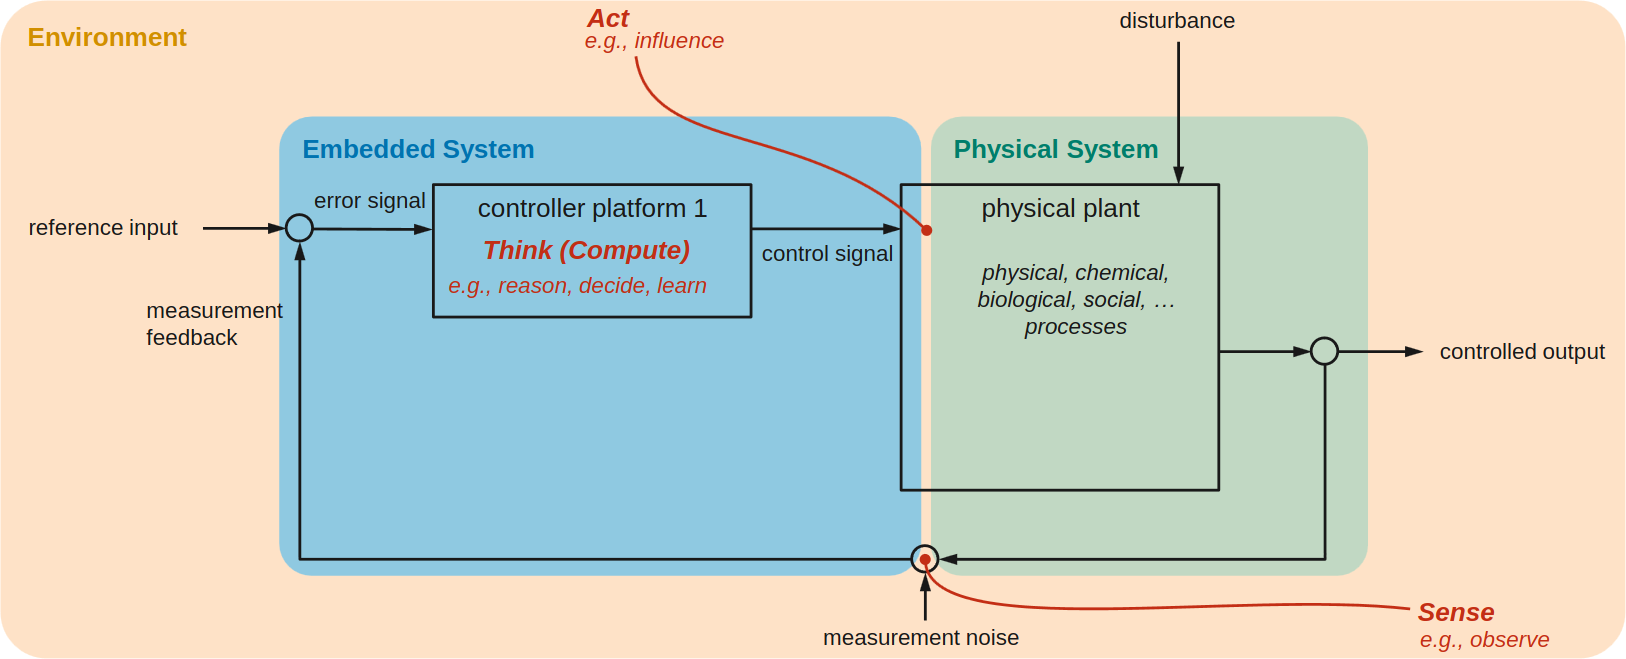
\includegraphics[width=\linewidth]{"Images/SenseThinkAct.png"}

Bei einem CPC (Cyber Physical System):

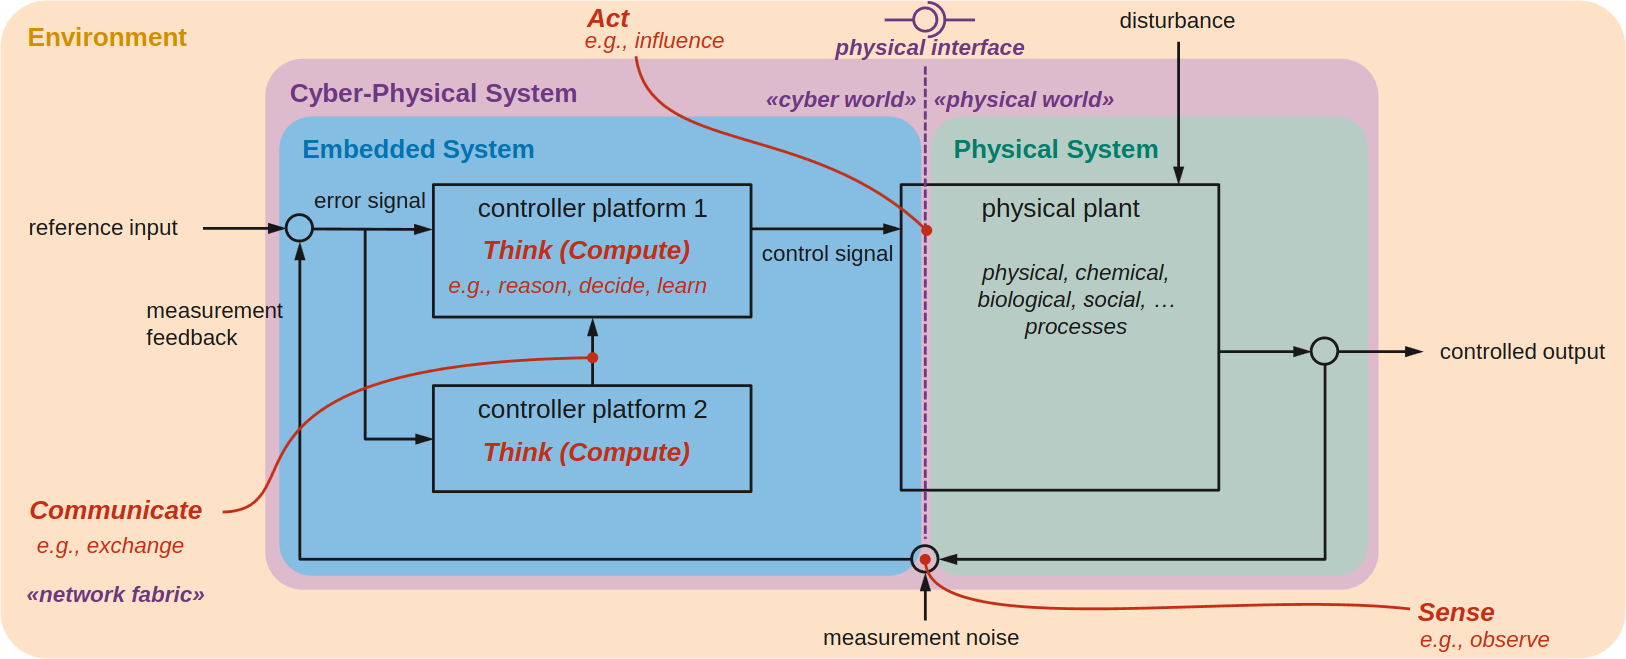
\includegraphics[width=\linewidth]{"Images/SenseThinkActCommunicate.png"}

\subsection{Schichtmodell}

\begin{center}
	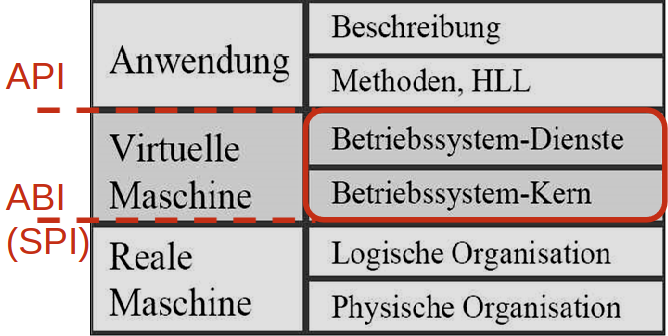
\includegraphics[width=.6\linewidth]{"Images/Schichtmodell.png"}
\end{center}

Das Betriebssystem im Schichtenmodell des Computersystems bietet der Anwendung API-Schnittstellen zur darunterliegenden realen Maschine und macht die Anwendung damit weitgehend unabhängig von der realen Maschine (CPU, Hardware, Peripherien,...).

\subsection{Entwicklungsprozess}

Unterschiedliche Möglichkeiten wie V-Modell und DevOps Lyfecycle (Loop).

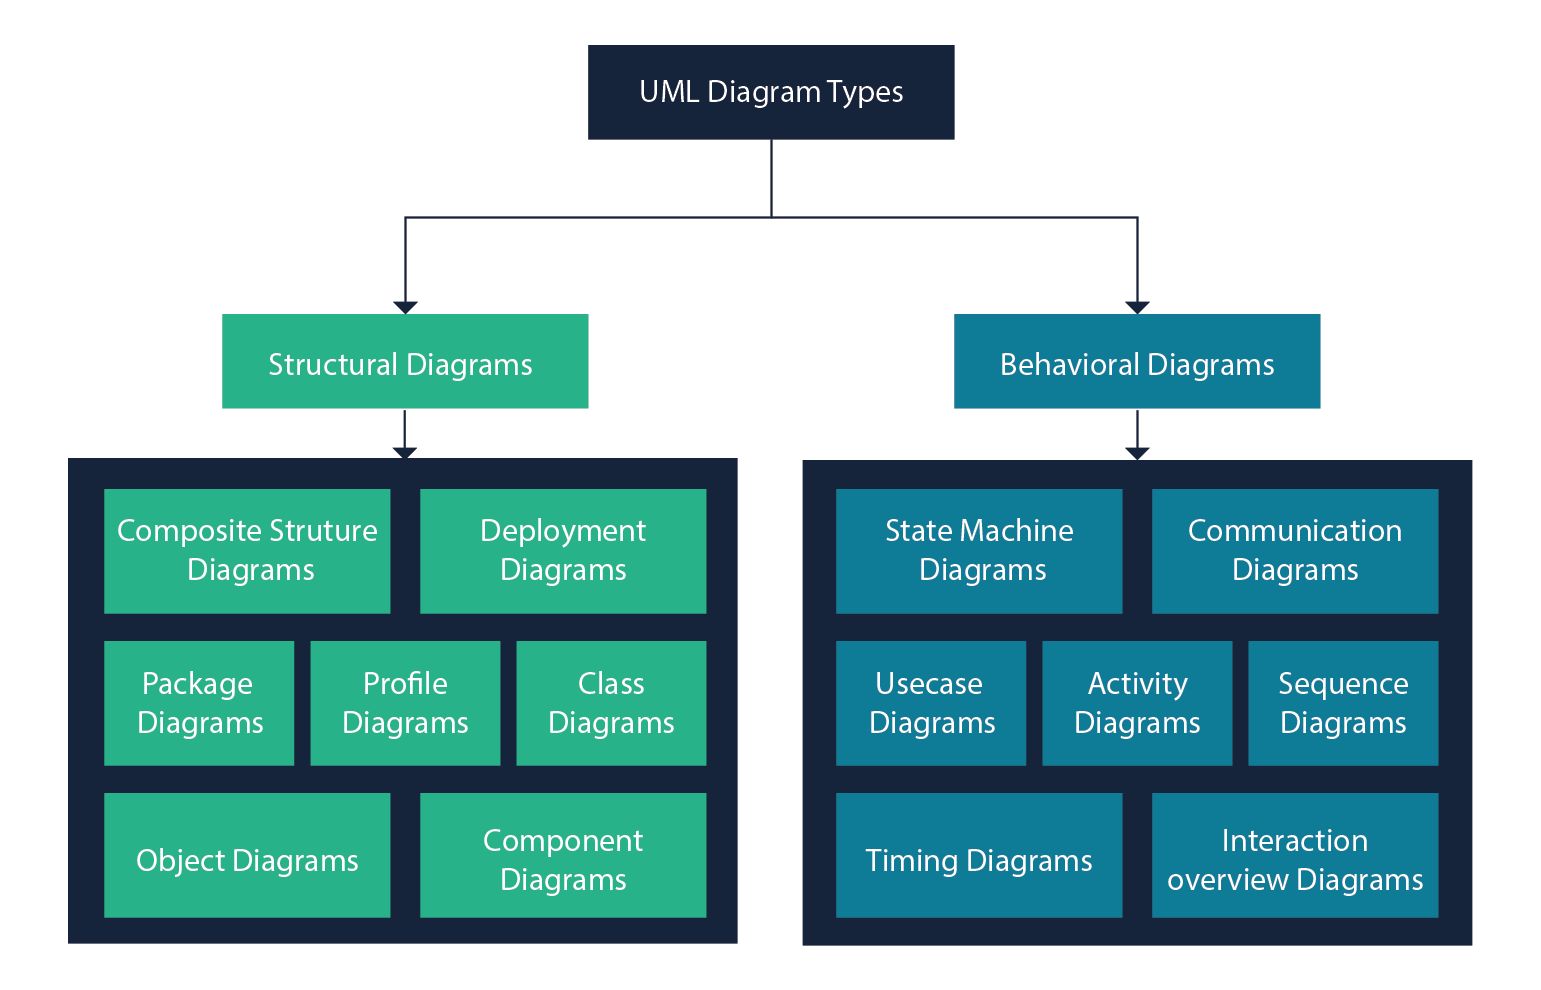
\includegraphics[width=\linewidth]{"Images/UML-Diagram-types-1.png"}

\subsection{Mikrocontroller-Organisation}

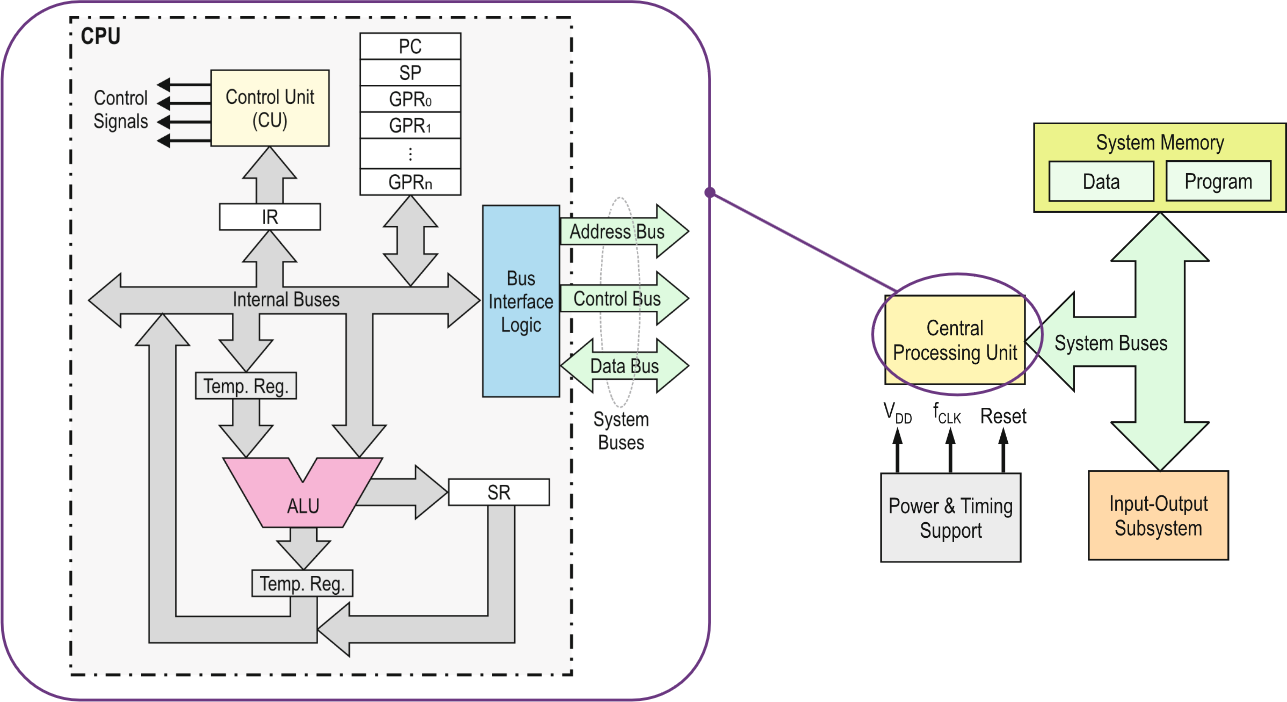
\includegraphics[width=\linewidth]{"Images/MikrocontrollerOrganisation.png"}

\subsubsection{System Komponenten}

\begin{itemize}
	\itemsep-.5em 
	\item \textit{NVIC}: Nested Vectored Interrupt Controller, provides configurable interrupt handling abilities to the processor.
	\item \textit{SYSTICK}: System timer, 24-bit down-counter, automatic reload.
	\item \textit{MPU}: Memory Protection Unit, Zugriffsregeln für Privileged Access und User Program Access, wirft Exceptions.
	\item \textit{FPU}: Floating Point Unit, erweiterter Befehlssatz auf DSP.
\end{itemize}

	\section{Betriebssysteme}

	\section{Interprozesskommunikation}

\subsection{Semaphore}

Semaphor ist ein Signalisierungsmechanismus (signaling mechanism), bestehend aus einer P-Operation (proberen, prüfen, reservieren) und V-Opration (verhogen, erhöhen, freigeben).

Binäre Semaphore:

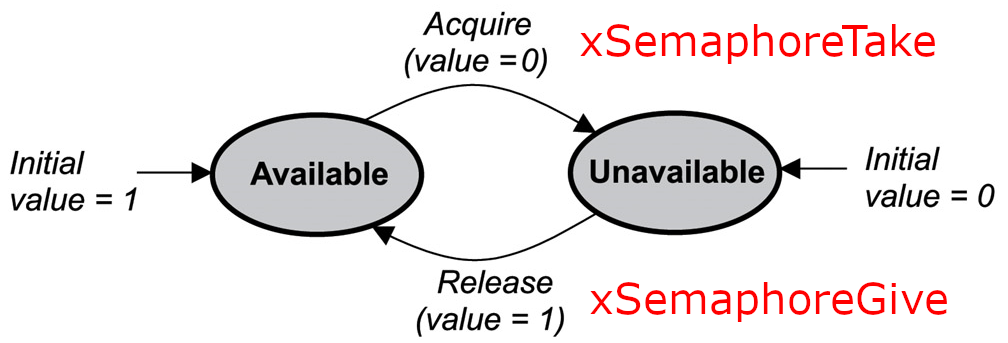
\includegraphics[width=.9\linewidth]{Binary_Semaphore.png}

Counting Semaphore:

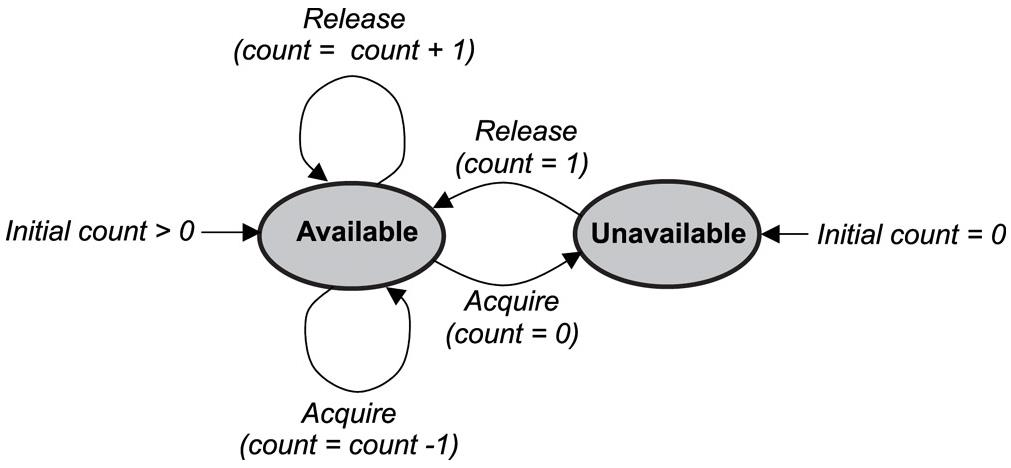
\includegraphics[width=\linewidth]{Counting_Semaphore.png}

\subsection{Mutual Exclusion (Mutex) Semaphore}

Die Mutex ist ein Sperrmechanismus (locking mechanism), welcher den Wert 0 und 1 annehmen kann.
Key words: Ownership, Recursive Locking, Task Deletion Safety, Priority Inversion Avoidance.
Recursive mutexes can be locked and unlocked multiple times by the task that owns them.

\subsection{Synchronisation}

\begin{center}
    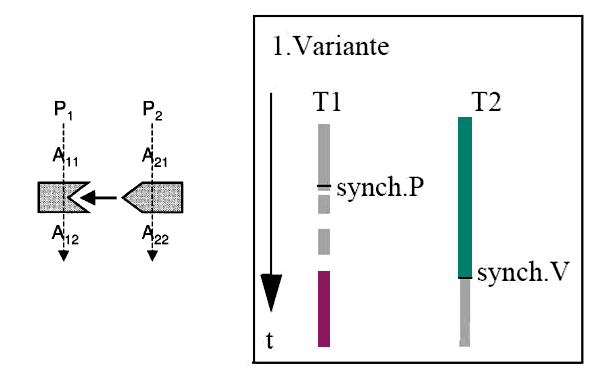
\includegraphics[width=.8\linewidth]{semaphore_sync1.png}

    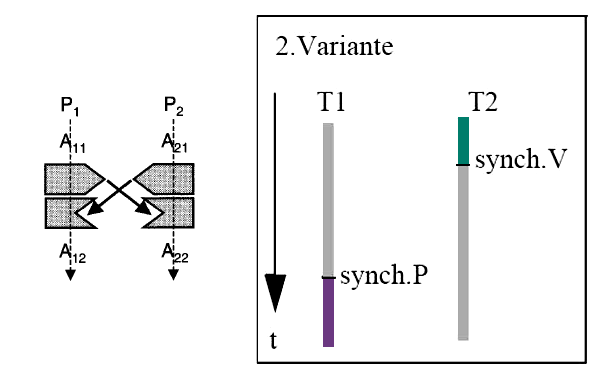
\includegraphics[width=.8\linewidth]{semaphore_sync2.png}
\end{center}


\subsection{Message Queues}

Eine Message Queue ist ein Buffer mit dem Tasks und ISR's Nachrichten austauschen und mit einander Kommuniziern können.

\subsubsection{Queue Control Block (QCB)}

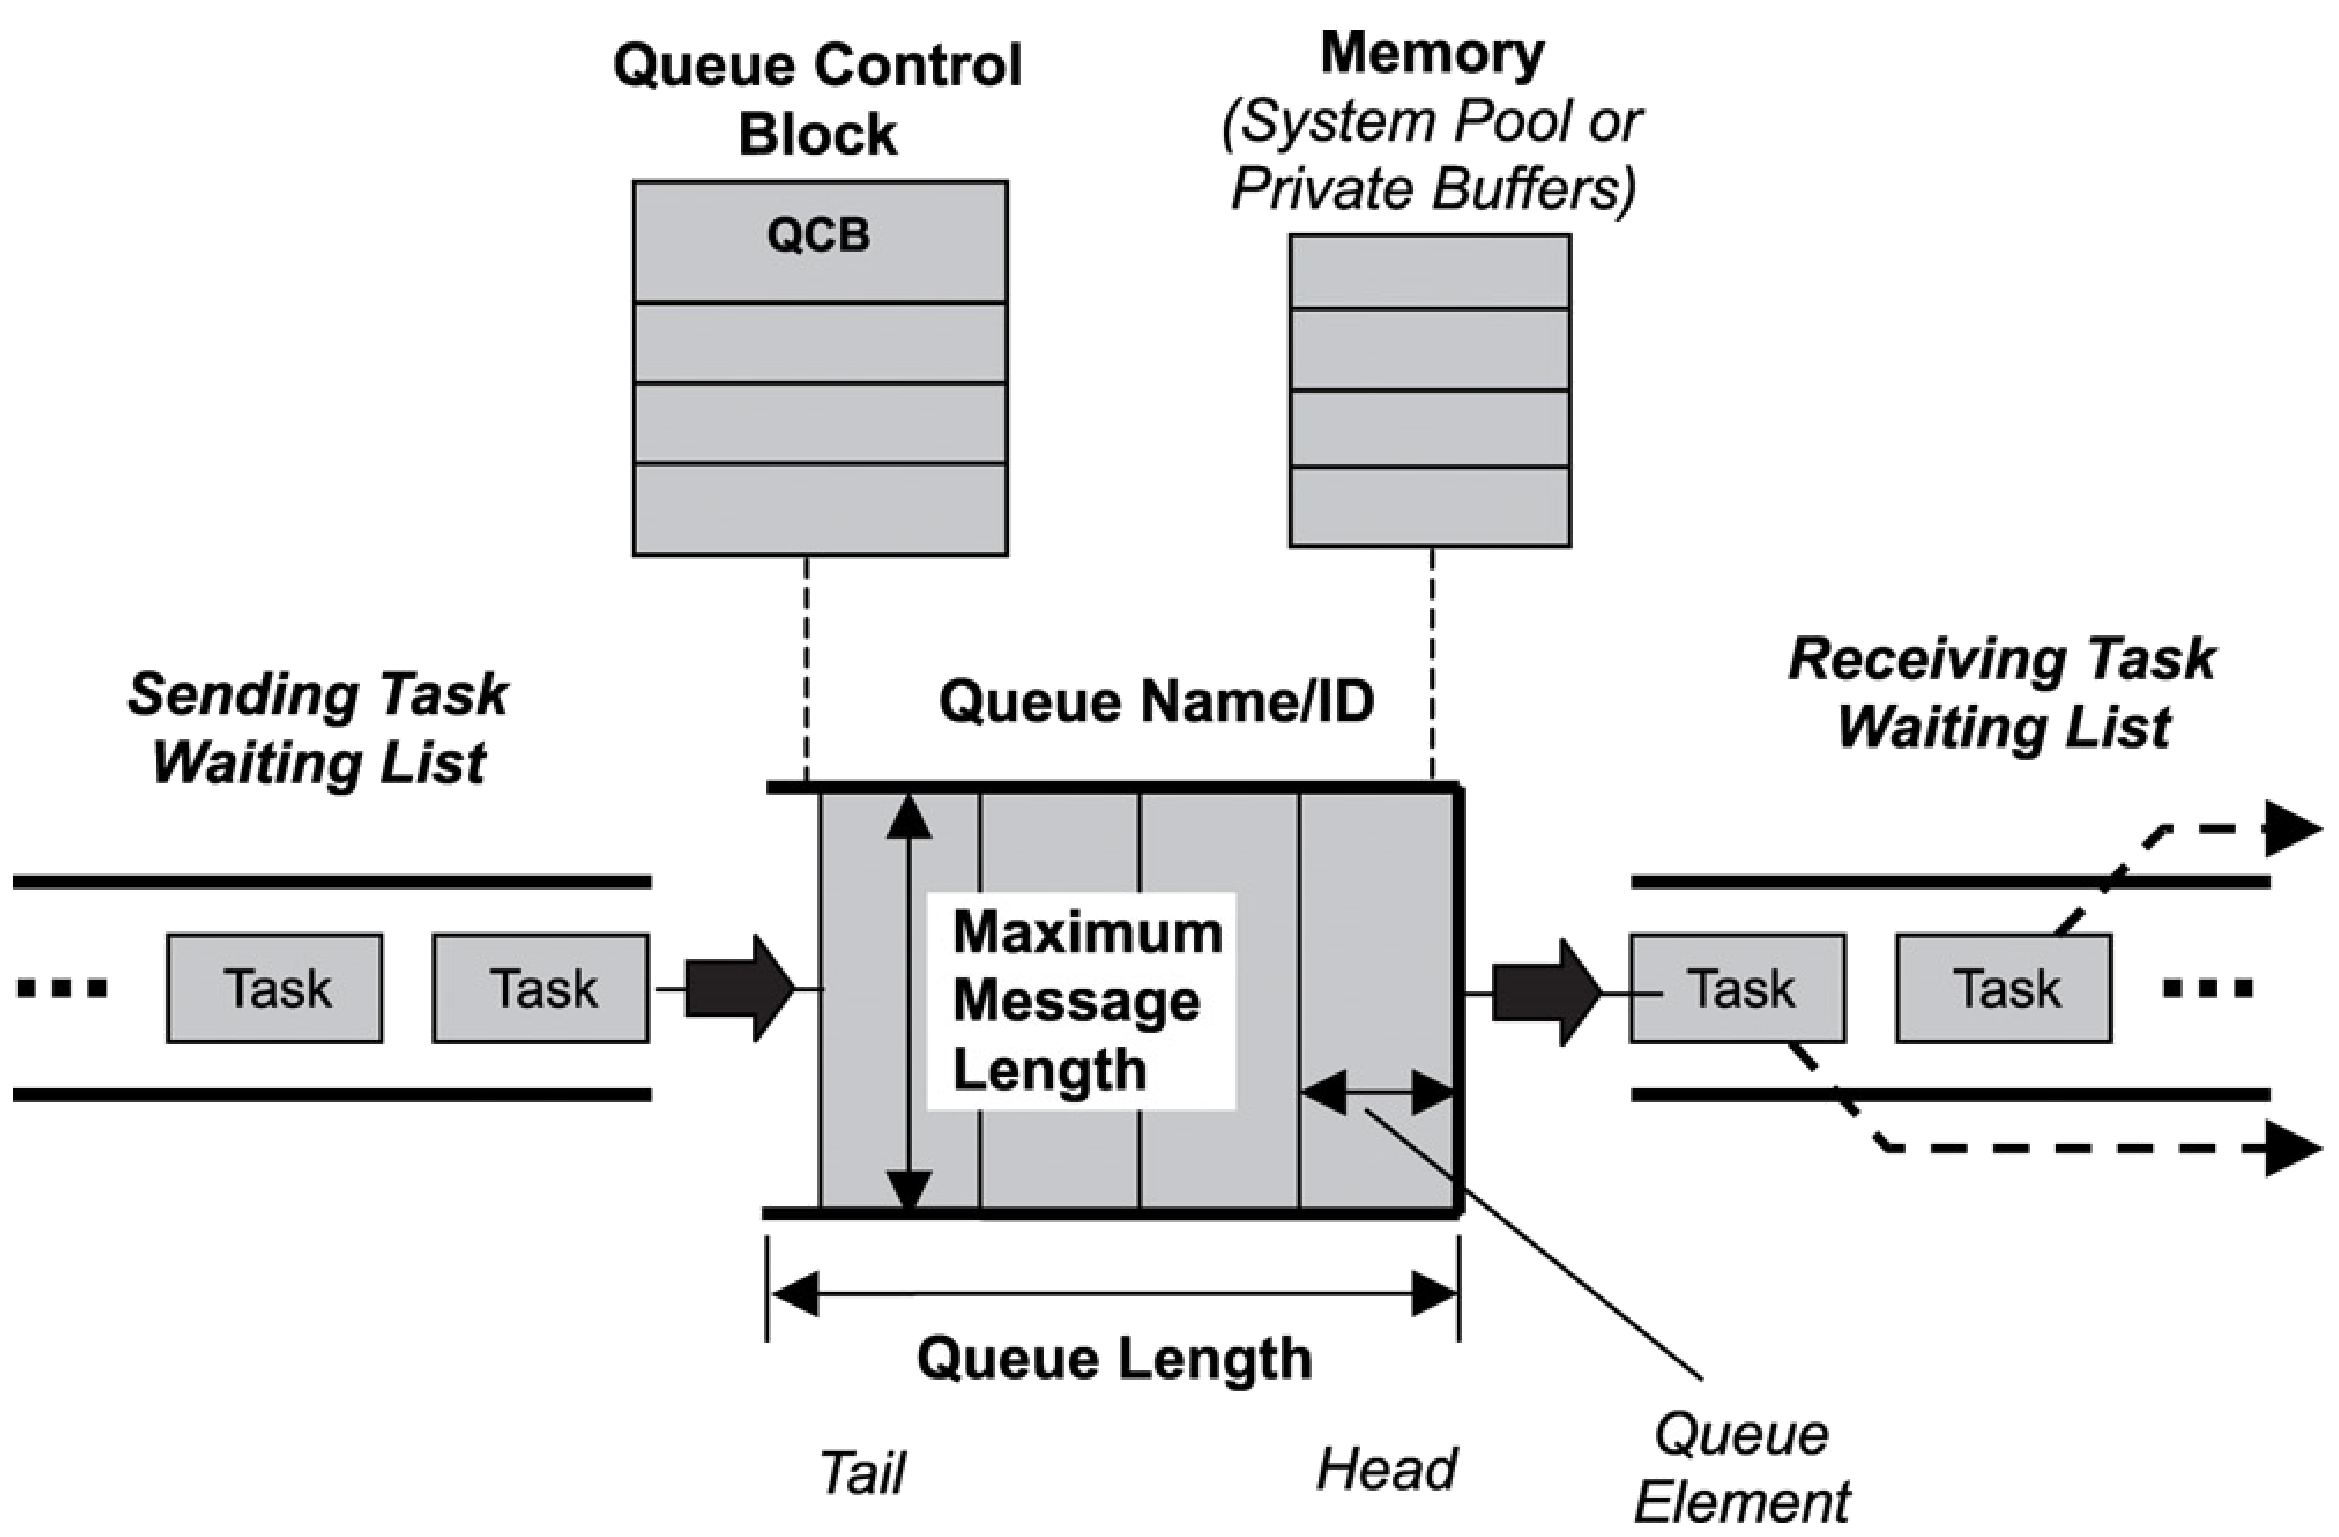
\includegraphics[width=\linewidth]{queue_control_block.png}

Zustandsdiagramm:

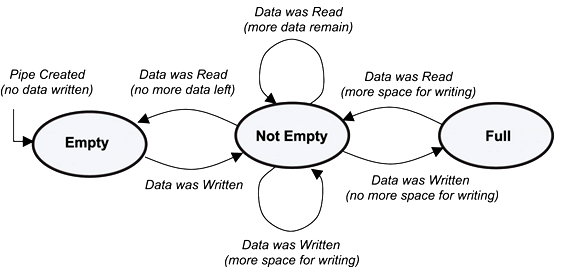
\includegraphics[width=\linewidth]{message_queue_zustandsdiagramm.png}

Unterschiedliche Kommunikationsmodelle möglich, wie One-Way Non-Interlocking und Interlocked, Two-Way Interlocked, Client-Server und Broadcast / Publish-Subscribe.


\subsubsection{Queue Set}

Queue Set ermöglicht einem RTOS Task simultan zu blockieren (pend) beim Lesezugriff auf
mehrere RTOS Queues und/oder Semaphore (block on set, not on individual object).


\subsubsection{Signals}

Ein Signal is ein Software-Interrupt welcher beim Signal-empfangenden Task einen asynchronen ablauf triggert / auslöst.
Signals can be ignored, made pending, processed (handled), or blocked.

Der \textbf{Singla Control Block} beinhaltet ein set der Signale, welche vom Task behandelt werden können.

In FreeRTOS sind Signale als \textit{Task Notifications} implementiert.


\subsubsection{Event Register, Event Groups}

Über das Event Register kann ein Task das Vorhandensein bestimmter Events prüfen,
die Einfluss auf dessen Ausführung haben können.
Eine externe Quelle, z.B. ein anderer Task oder ein ISR kann Bits im Event Register setzen,
um den Task zu informieren, dass ein bestimmter Event eingetreten ist.
Der \textbf{Event Register Control Block} ist ein Teil des \textbf{Task Control Blocks} (TCB).

In FreeRTOS is eine Event Group eine Menge von Event-Bits.
Einzelne Event-Bits innerhalb einer Event Group werden durch eine Bit-Nummer referenziert.

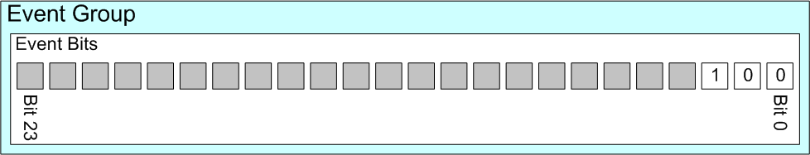
\includegraphics[width=\linewidth]{EventGroup.png}

\subsubsection{Pipes}

Pipes sind Kernel Objekte welche einen unstrukturierten Datenaustausch und Synchronisation zwischen den tasks ermöglicht.
Es können Mehrer Tasks in die pipe schreiben und auch mehrere daraus Lesen.
Pipes werden dynamisch erzeugt und gelöscht, wobei vom Kernel ein Pipe Control Block und zwei waiting lists zugewiesen werden.

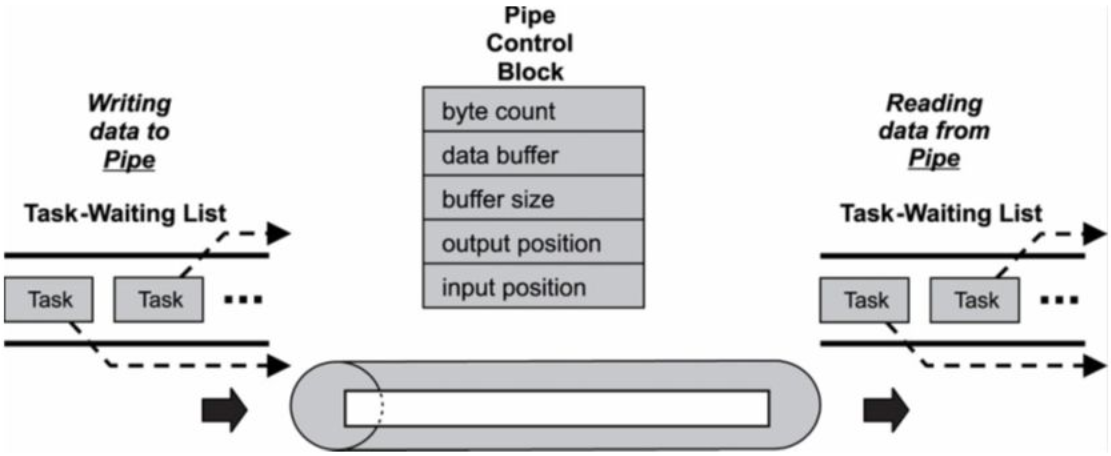
\includegraphics[width=\linewidth]{pipe_overview.png}

In FreeRTOS sind Pipes so nicht direkt vorhanden, alternativen sind Queues, Stream Buffers und Message Buffers.
	\section{Deadlocks und Priority Inversion}

Bei überlappender oder zyklischer Belegung von Betriebsmitteln (Ressourcen) können Verklemmungen (Deadlocks) auftreten.
\textbf{Race Condition}: unerwünschtes Wettrennen mehrere Tasks um gleichzeitigen Zugriff auf Ressource.
Ein Deadlock ist immer die Folge eines logischen Programmfehlers!

Eine Möglichkeit um Deadlocks erkennen zu können ist der Prozessfahrplan:

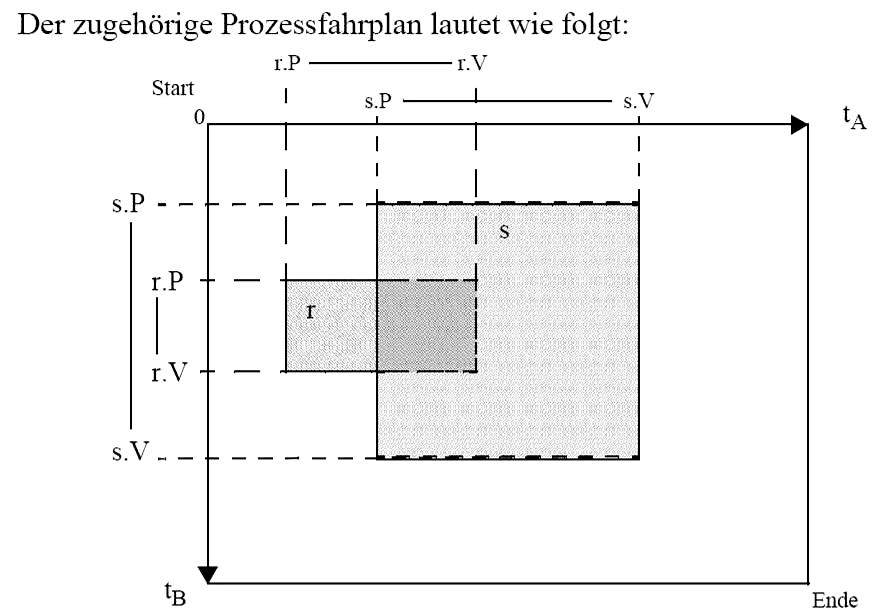
\includegraphics[width=\linewidth]{Prozessfahrplan.png}

Methoden zum verhindern von Deadlocks:

\begin{itemize}
    \itemsep-.5em 
    \item Eliminate the \textit{no preemption} deadlock condition: Task must release already acquired resources if a new request is denied. Task must then initiate a new request, including both the new resource and all previously held resources.
    \item Eliminate the \textit{hold and wait} deadlock condition: Task requests at one time all needed resources; it can begin execution only when every resource from the request set is granted.
    \item Eliminate the \textit{circular wait} deadlock condition: All tasks shall request the resources in the very same numbering according to an imposed ordering on the resources.
\end{itemize}


\subsection{Priority Inversion}

Wenn ein Low priority Task eine Resource blockiert welche von eine high Priority Task benötigt wird.

Bounded Priority Inversion:

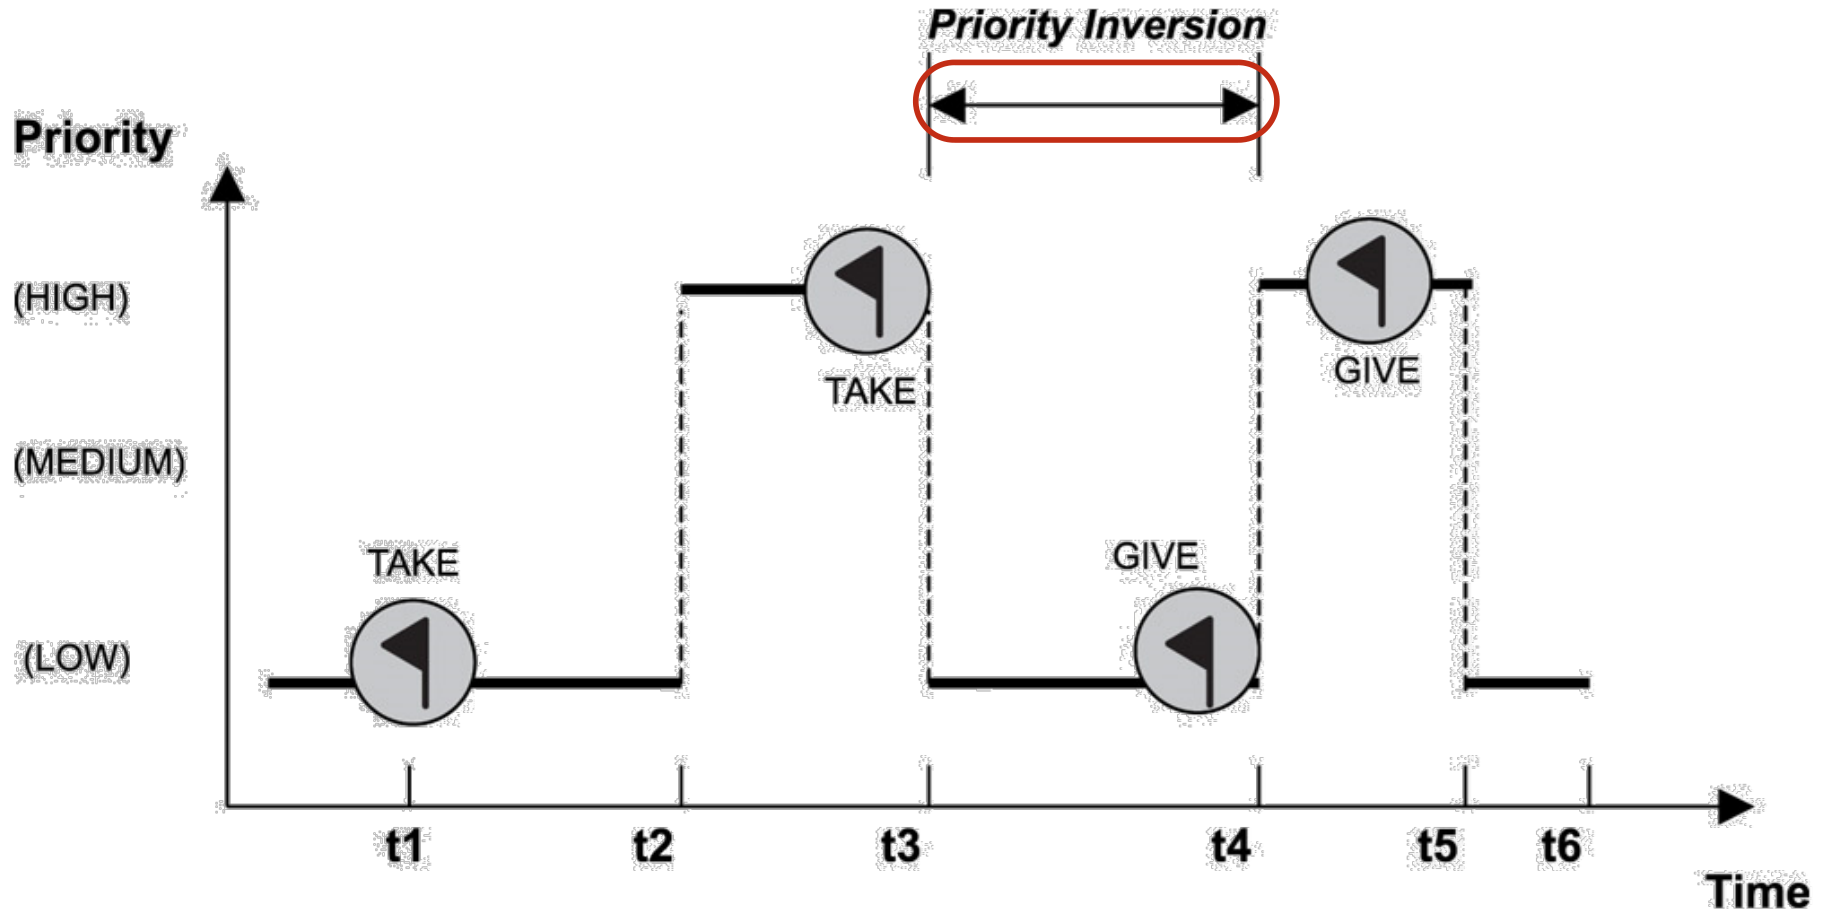
\includegraphics[width=\linewidth]{BoundedPriorityInversion.png}

Unbounded Priority Inversion:

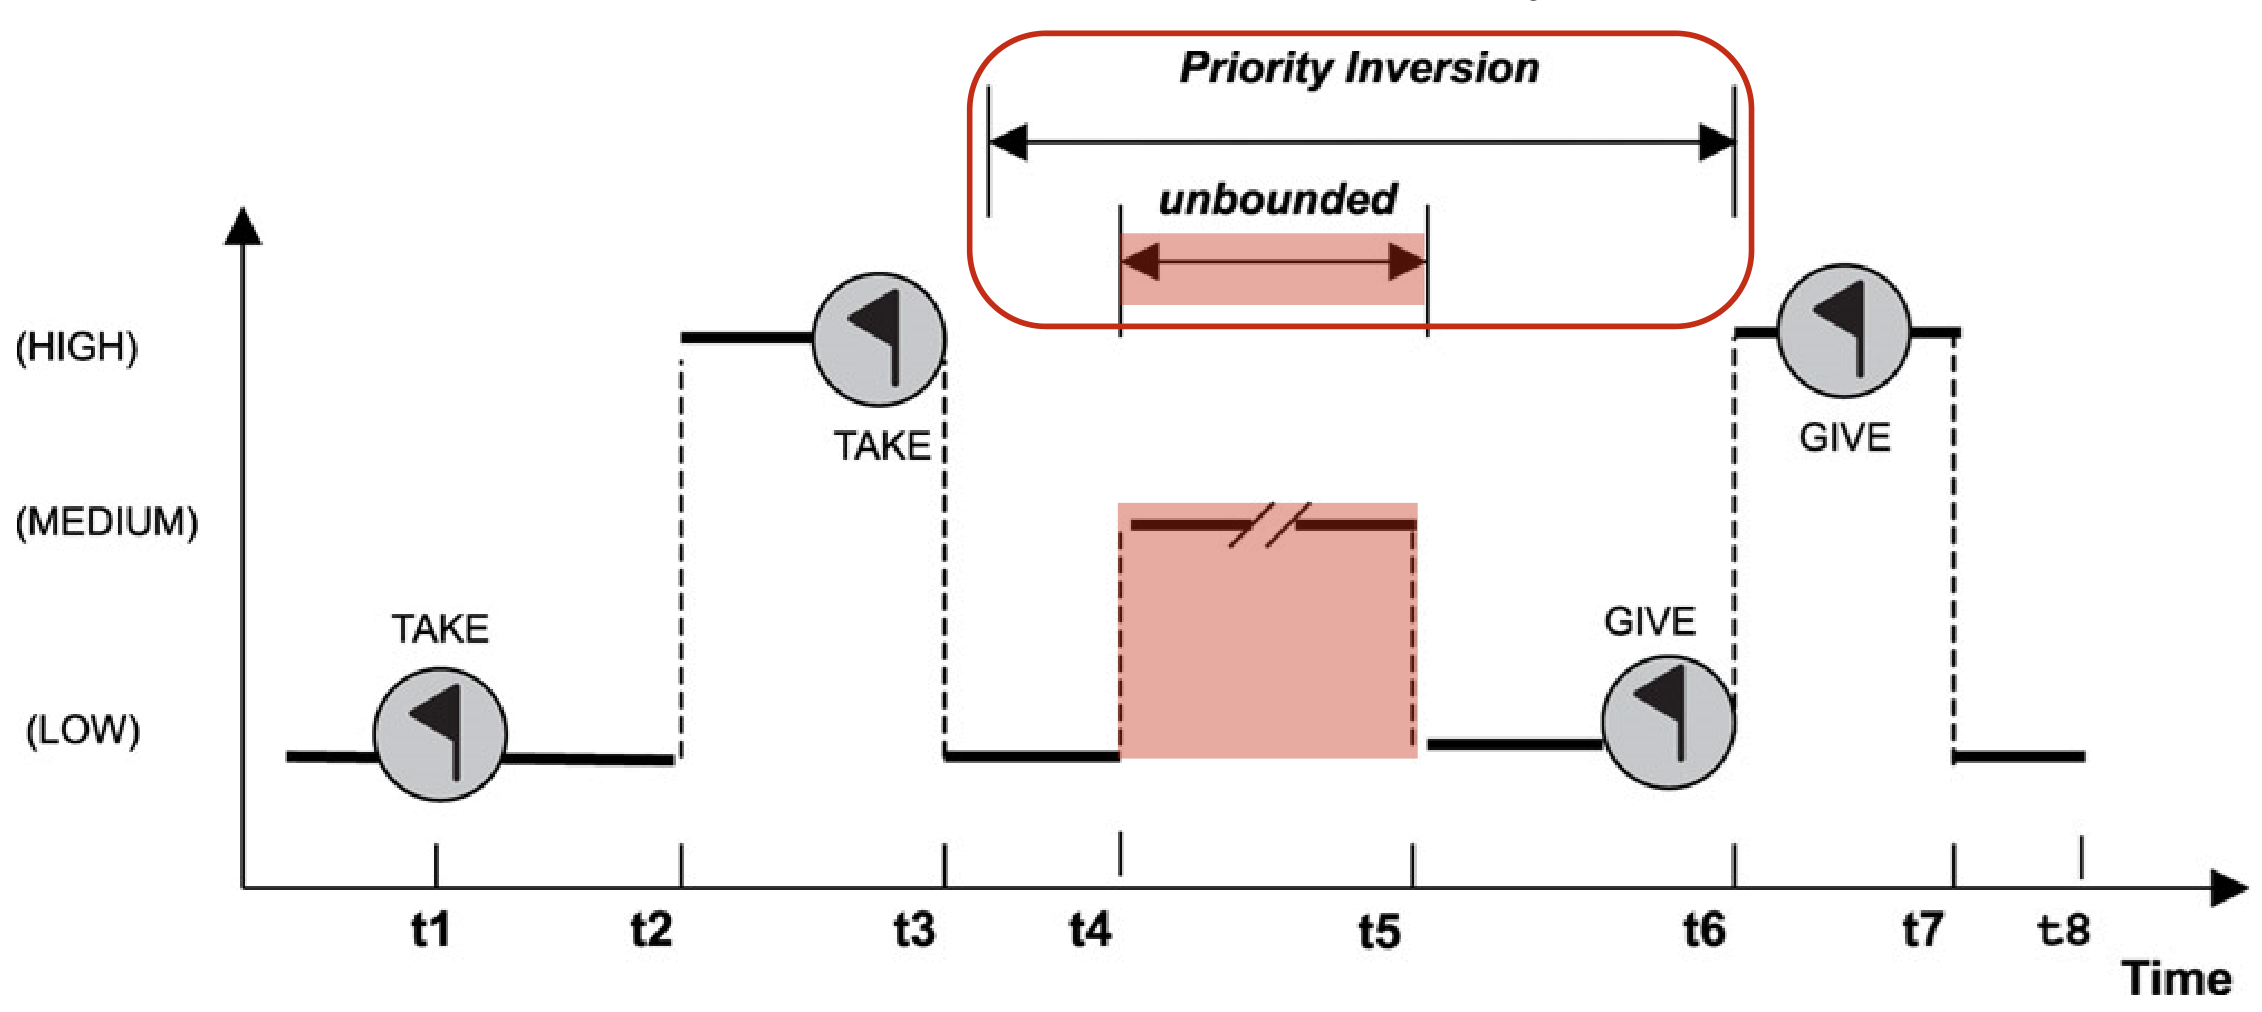
\includegraphics[width=\linewidth]{UnboundedPriorityInversion.png}

\subsubsection{Priority Inheritance Protocol (PIP)}

Erhöht die priorität des LPT zu der des HPT damit die Resource schneller freigegeben wird.

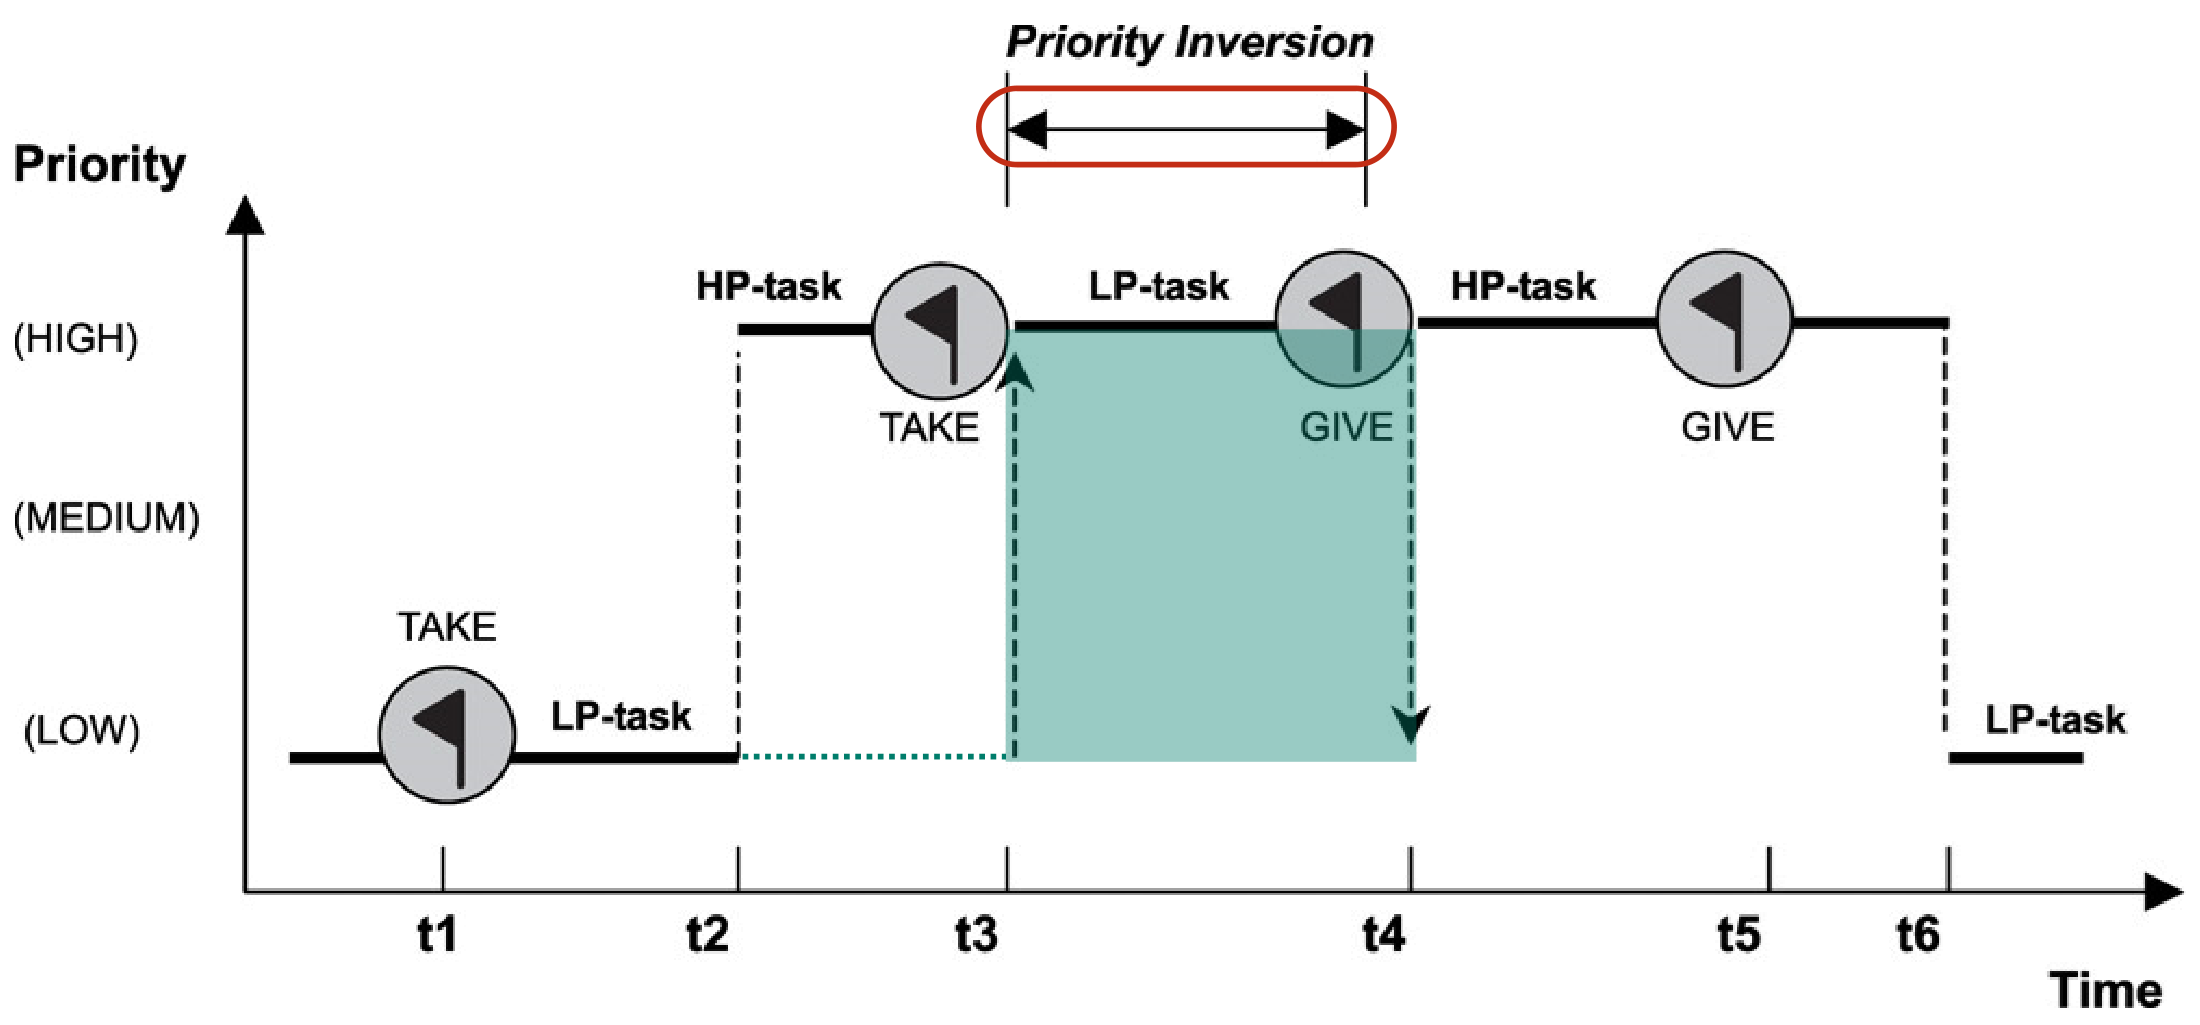
\includegraphics[width=\linewidth]{PriorityInheritanceProtocol.png}

\subsubsection{Transitive Priority Promotion}

Der "transitive" Teil bedeutet, dass diese Prioritätsbeförderung nicht nur zwischen zwei Tasks stattfindet, sondern sich über mehrere Ebenen von wartenden Tasks ausbreiten kann.

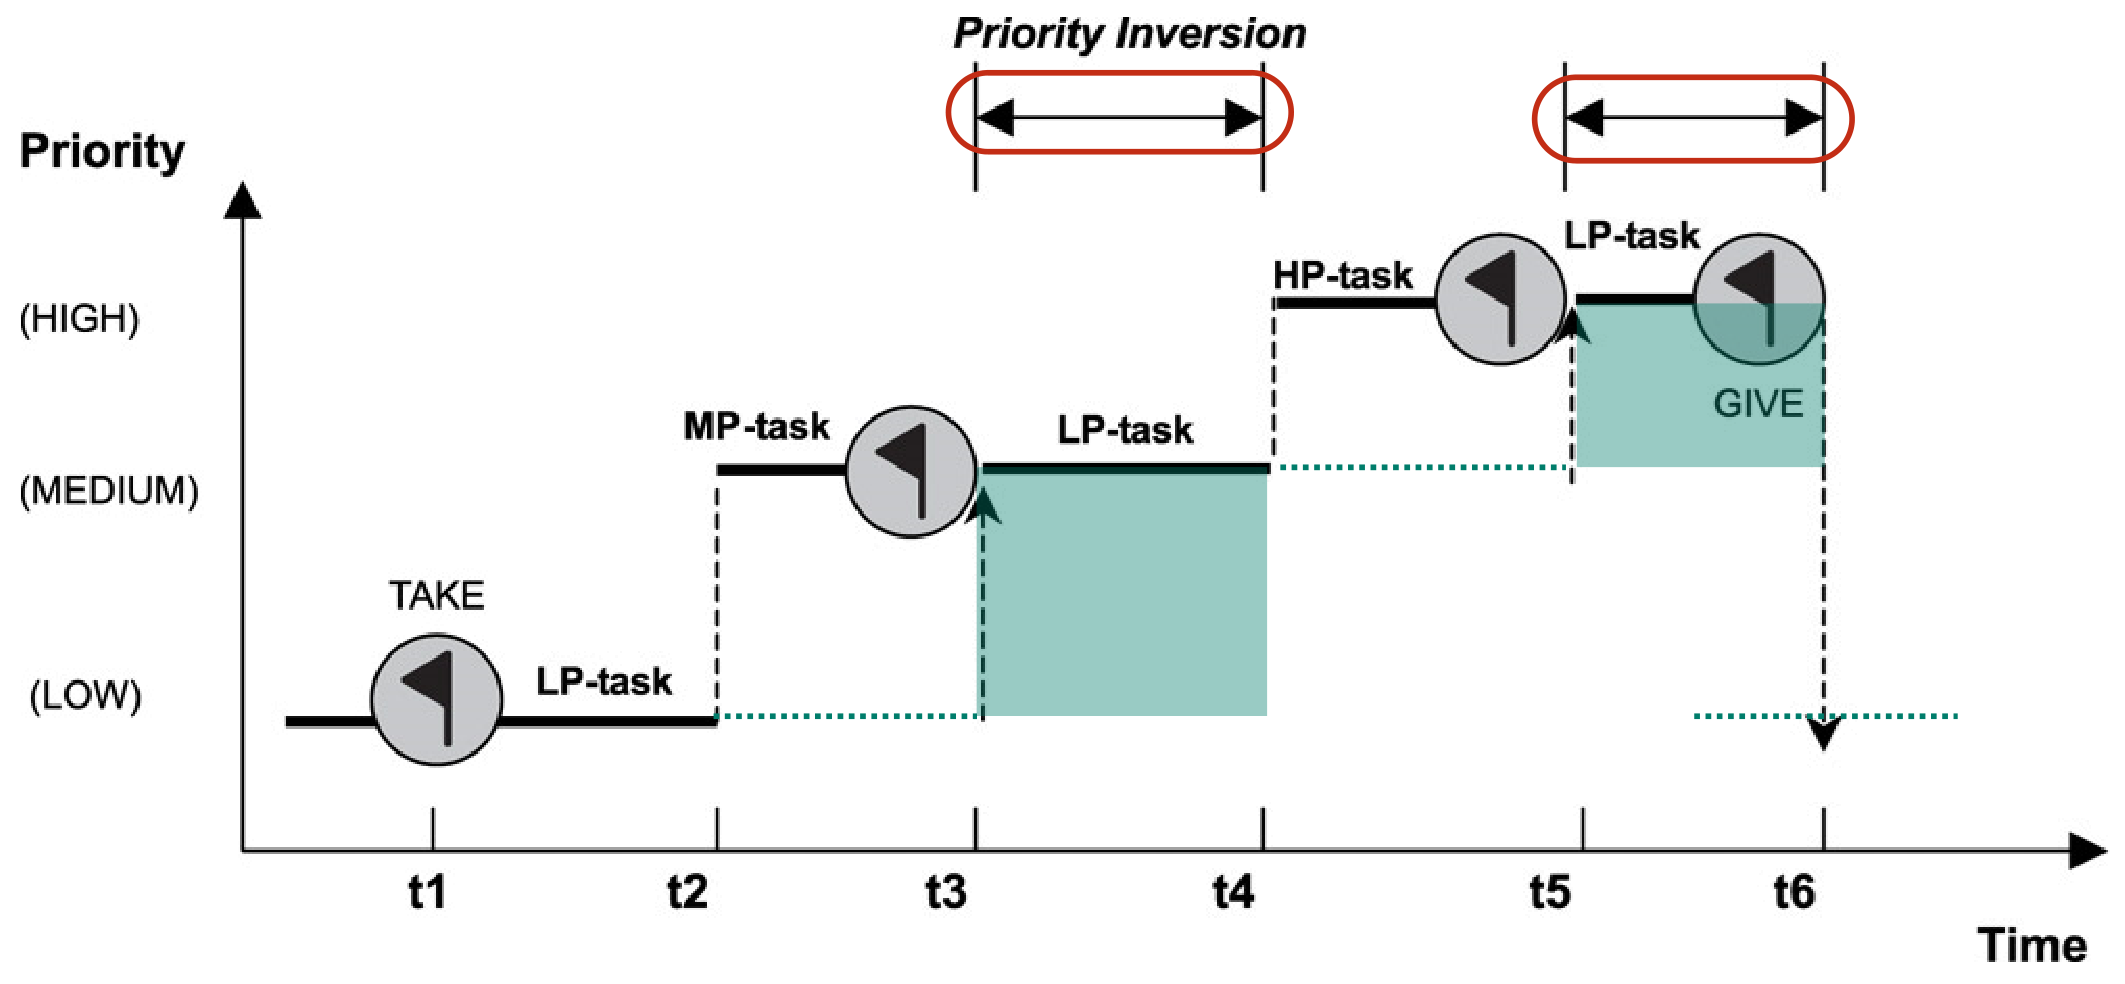
\includegraphics[width=\linewidth]{TransitivePriorityPromoton.png}

\subsubsection{Priority Ceiling Protocol (PCP)}

\underline{Variante 1, Regeln:}

Task erhält direkt die Highest priority ceiling Priorität der Resource.

\begin{itemize}
    \itemsep-.5em 
    \item If resource locked, task blocks.
    \item If resource free, task takes and locks it; task's priority raised to resource's priority ceiling.
    \item When resource released, task's priority is assigned to highest priority of remaining resources held.
\end{itemize}

\underline{Variante 2, Regeln:}

Current priority ceiling = highest priority ceiling of all resources in use at given time.

\begin{itemize}
    \itemsep-.5em 
    \item If resource locked, task blocks
    \item If resource free and task's priority > current priority ceiling, task takes and locks it, else
    \item If current priority ceiling stems from another resource the task currently already holds, task can also take and lock this resource, else task blocks.
    \item Blocked task passes on its priority to other blocking task (priority inherited if higher); if that other blocking task releases a resource, it assumes highest priority among all tasks still blocked by resources held; if not blocking any other task, task returns to normal priority.
\end{itemize}



	\section{Scheduling}

\subsection{Rate Monotonic Scheduling (RM)}

Annahme:

\begin{itemize}
    \itemsep-.5em 
    \item All tasks that have hard deadlines are periodic.
    \item All tasks are independent.
    \item $d_i = p_i$ for all tasks.
    \item $c_i$ is constant and is known for all tasks.
    \item The time required for context switching is negligible.
\end{itemize}

\begin{minipage}[t]{.49\linewidth}
    \vspace{0pt}
    \formula{$\mu = \sum_{i=1}^{n}{\dfrac{c_i}{p_i}} \leq n ( \sqrt[n]{2} - 1 ) $}

    \unitText{$\mu$}{Auslastung}{1}\\
    \unitText{$n$}{Anzahl der Jobs}{1}\\
    \unitText{$c_i$}{Ausführungszeiten}{s}\\
    \unitText{$p_i$}{Periodenlängen}{s}
\end{minipage}\hfill
\begin{minipage}[t]{.25\linewidth}
    \vspace{0pt}
    \begin{tabular}{ c|c }
        $n$ & $\mu$ \\
        \hline
        1 & 1     \\
        2 & 0.828 \\  
        3 & 0.780 \\
        4 & 0.757 \\
       \end{tabular}
\end{minipage}\hfill
\begin{minipage}[t]{.25\linewidth}
    \vspace{0pt}
    \begin{tabular}{ c|c }
        $n$ & $\mu$ \\
        \hline
        5 & 0.743 \\
        6 & 0.734 \\
        7 & 0.728 \\
        8 & 0.724 \\
       \end{tabular}
\end{minipage}

Priorität: Kürzeste $c_i$, dann kürzeste $p_i$.


\subsection{Deadline Monotonic Scheduling (DM)}

\begin{minipage}[t]{.49\linewidth}
    \vspace{0pt}
    \formula{$\mu = \sum_{i=1}^{n}{\dfrac{c_i}{d_i}} \leq n ( \sqrt[n]{2} - 1 ) $}
\end{minipage}\hfill
\begin{minipage}[t]{.49\linewidth}
    \vspace{0pt}
    \unitText{$\mu$}{Auslastung}{1}\\
    \unitText{$n$}{Anzahl der Jobs}{1}\\
    \unitText{$c_i$}{Ausführungszeiten}{s}\\
    \unitText{$d_i$}{Deadline}{s}
\end{minipage}

Priorität: Kürzeste $c_i$, dann kürzeste $d_i$, dann kürzeste $p_i$.

\subsection{Earliest Deadline First (EDF)}

Es ordnet den Tasks Prioritäten zu, die sich nach der absoluten Deadline richten. Der Task, dessen Frist am nächsten ist, erhält die höchste Priorität.
Preemption möglich!

\begin{center}
    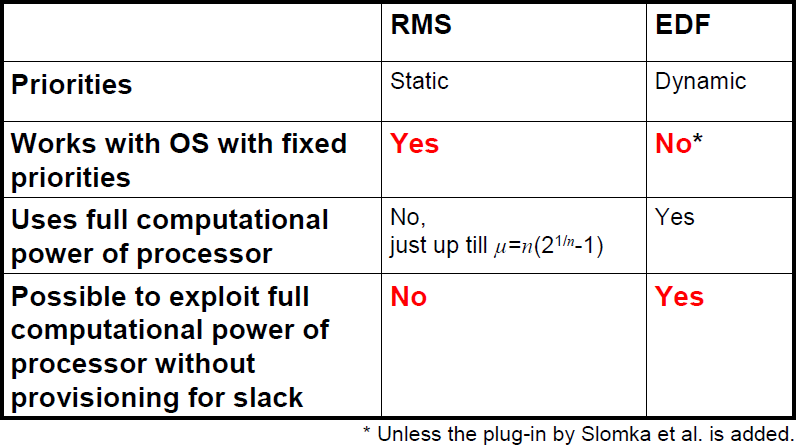
\includegraphics[width=.8\linewidth]{RMSvsEDF.png}
\end{center}


Oft werden Hybride verwendet:
\begin{center}
    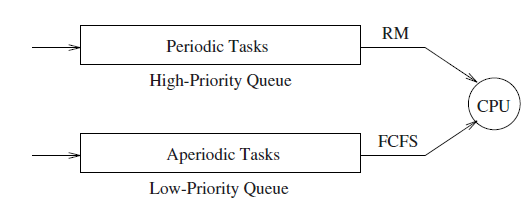
\includegraphics[width=.8\linewidth]{Scheduling_Hybrid.png}
\end{center}
	\section{Speicherhierarchie}

\begin{center}
    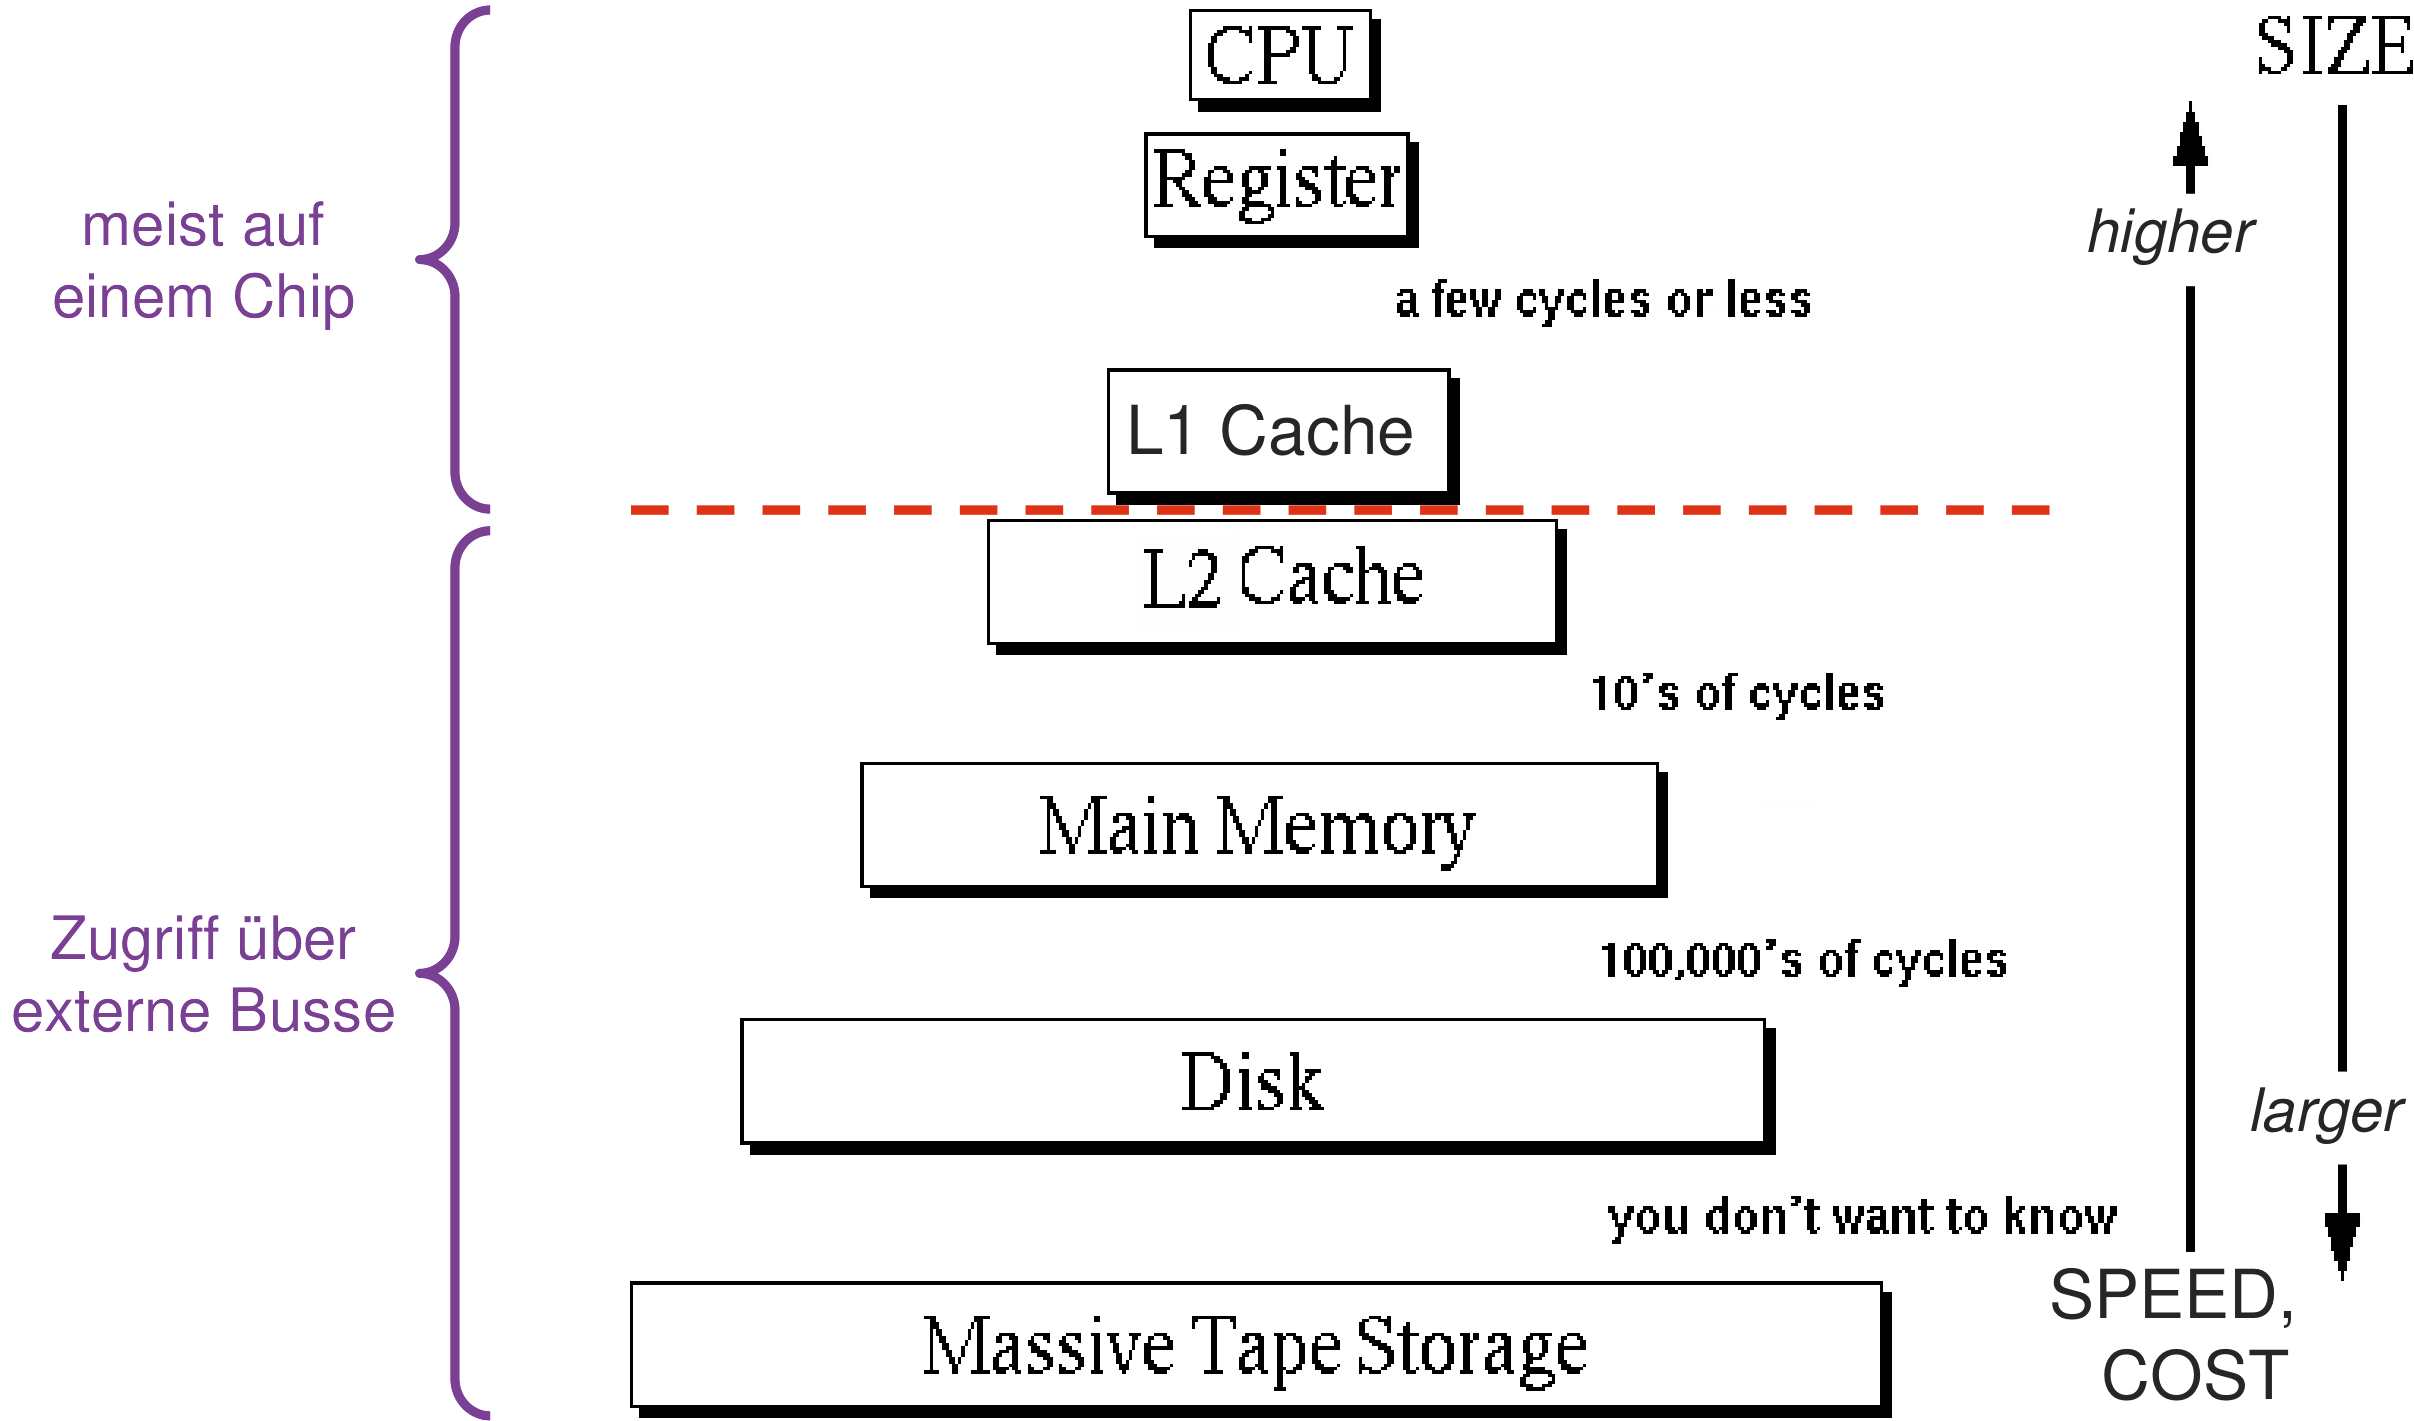
\includegraphics[width=.8\linewidth]{Speicherhierarchie.png}
\end{center}

\subsection{Cache-Speicher}

\begin{itemize}
    \itemsep-.5em 
    \item L1-Cache: auf gleichem Chip wie CPU, arbeiten mit der CPU-Geschwindigkeit, typisch bis etwa 128 KByte
    \item L2-, L3-Cache: ausserhalb des CPU-Chips, wesentlich langsamer als L1-Cache, L2 typisch 256 KByte bis mehrere MByte
\end{itemize}

Es gilt das Lokalitätsprinzip: Kopien von häufig (zeitliche Lokalität der Programmausführung) oder miteinander (örtliche Lokalität) benötigten Instruktionen/Daten aus dem Hauptspeicher.
Cache-Speicher (Daten, Adressen) und Cache-Controller (Steuersignal); Cache für den Prozessor versteckt, Programm läuft mit und ohne Cache.

Das Cache Directory ist als Assoziativ-Speicher aufgebaut, Content Addressable Memory (CAM):

\begin{center}
    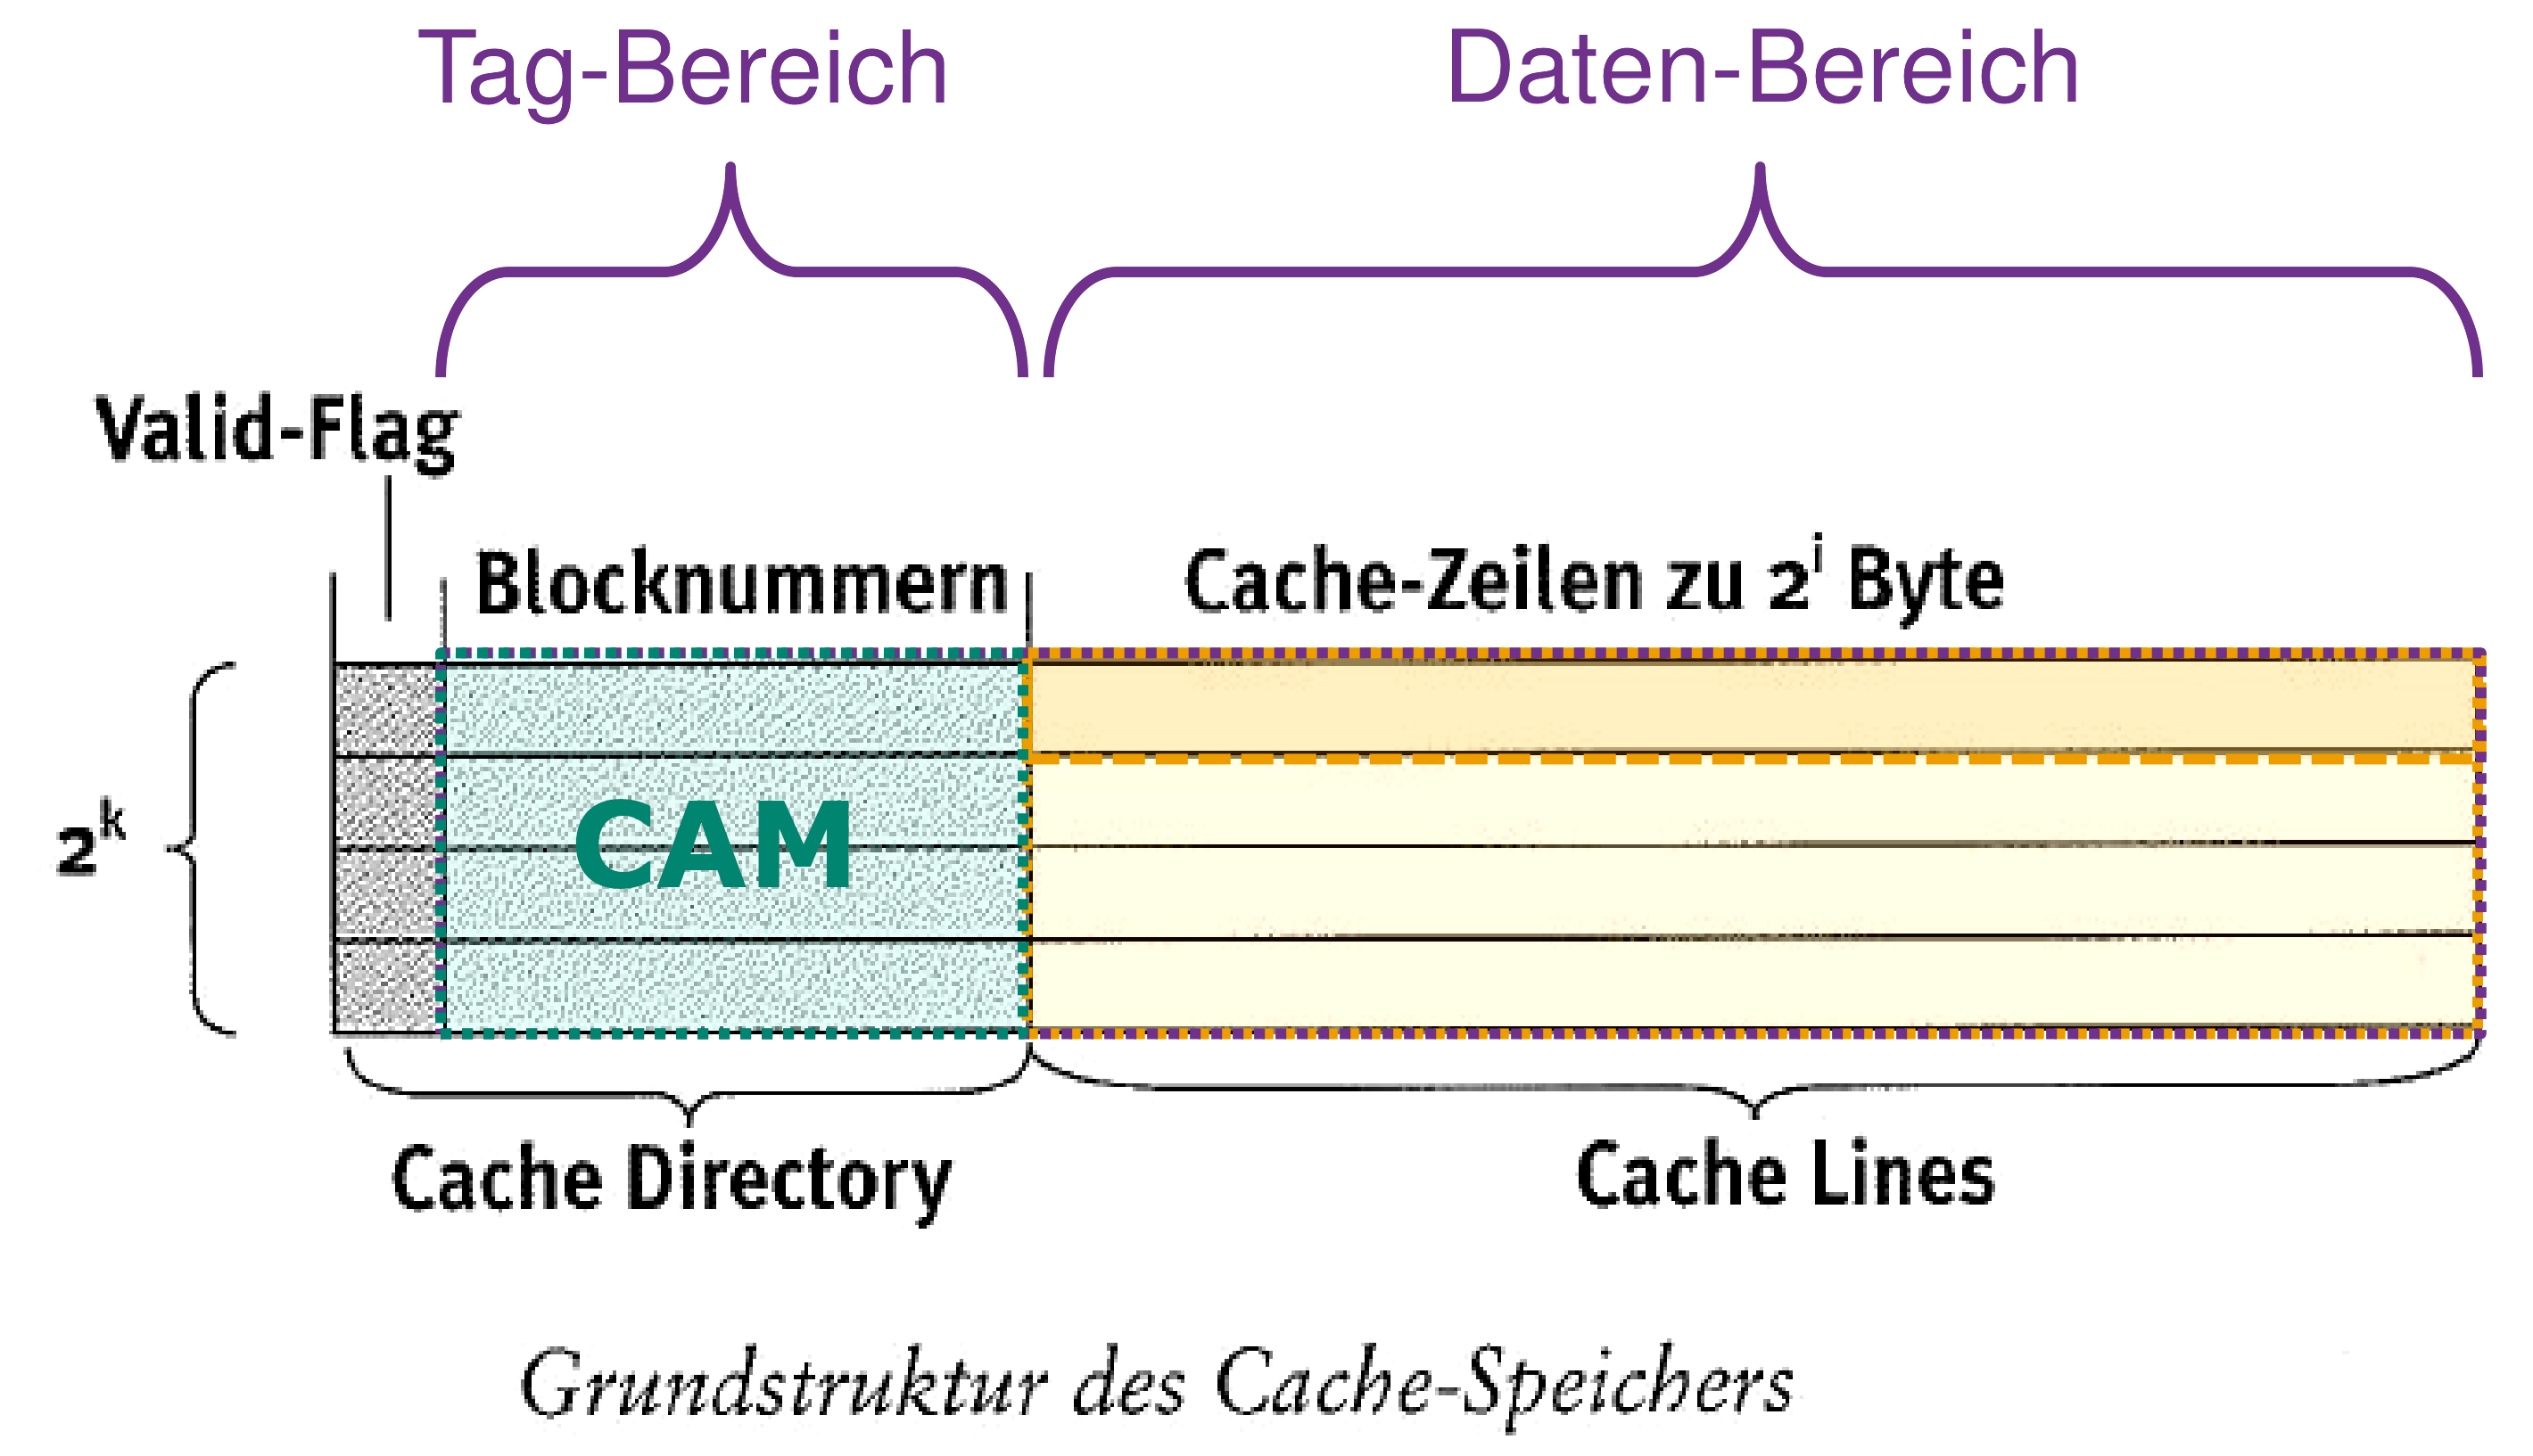
\includegraphics[width=.8\linewidth]{cache_cam.png}
\end{center}

\subsection{Cache Organisation}

\subsubsection{Voll-assoziativ}

Die Dateneinheit kann sich an beliebiger Stelle im Cache befinden.
Beim CAM-Zugriff sind $2^k$ Vergleiche gleichzeitig in der Cache-Hardware durchzuführen.

Übung: Kontinuierlich von Vorne her aufgefüllt (Start Zeile 0)

Cache Grösse: \formula{$2^{k+i}$}
Anzahl Zeilen: \formula{$2^k$}
Zeilen-Grösse: \formula{$2^i$}

\begin{center}
    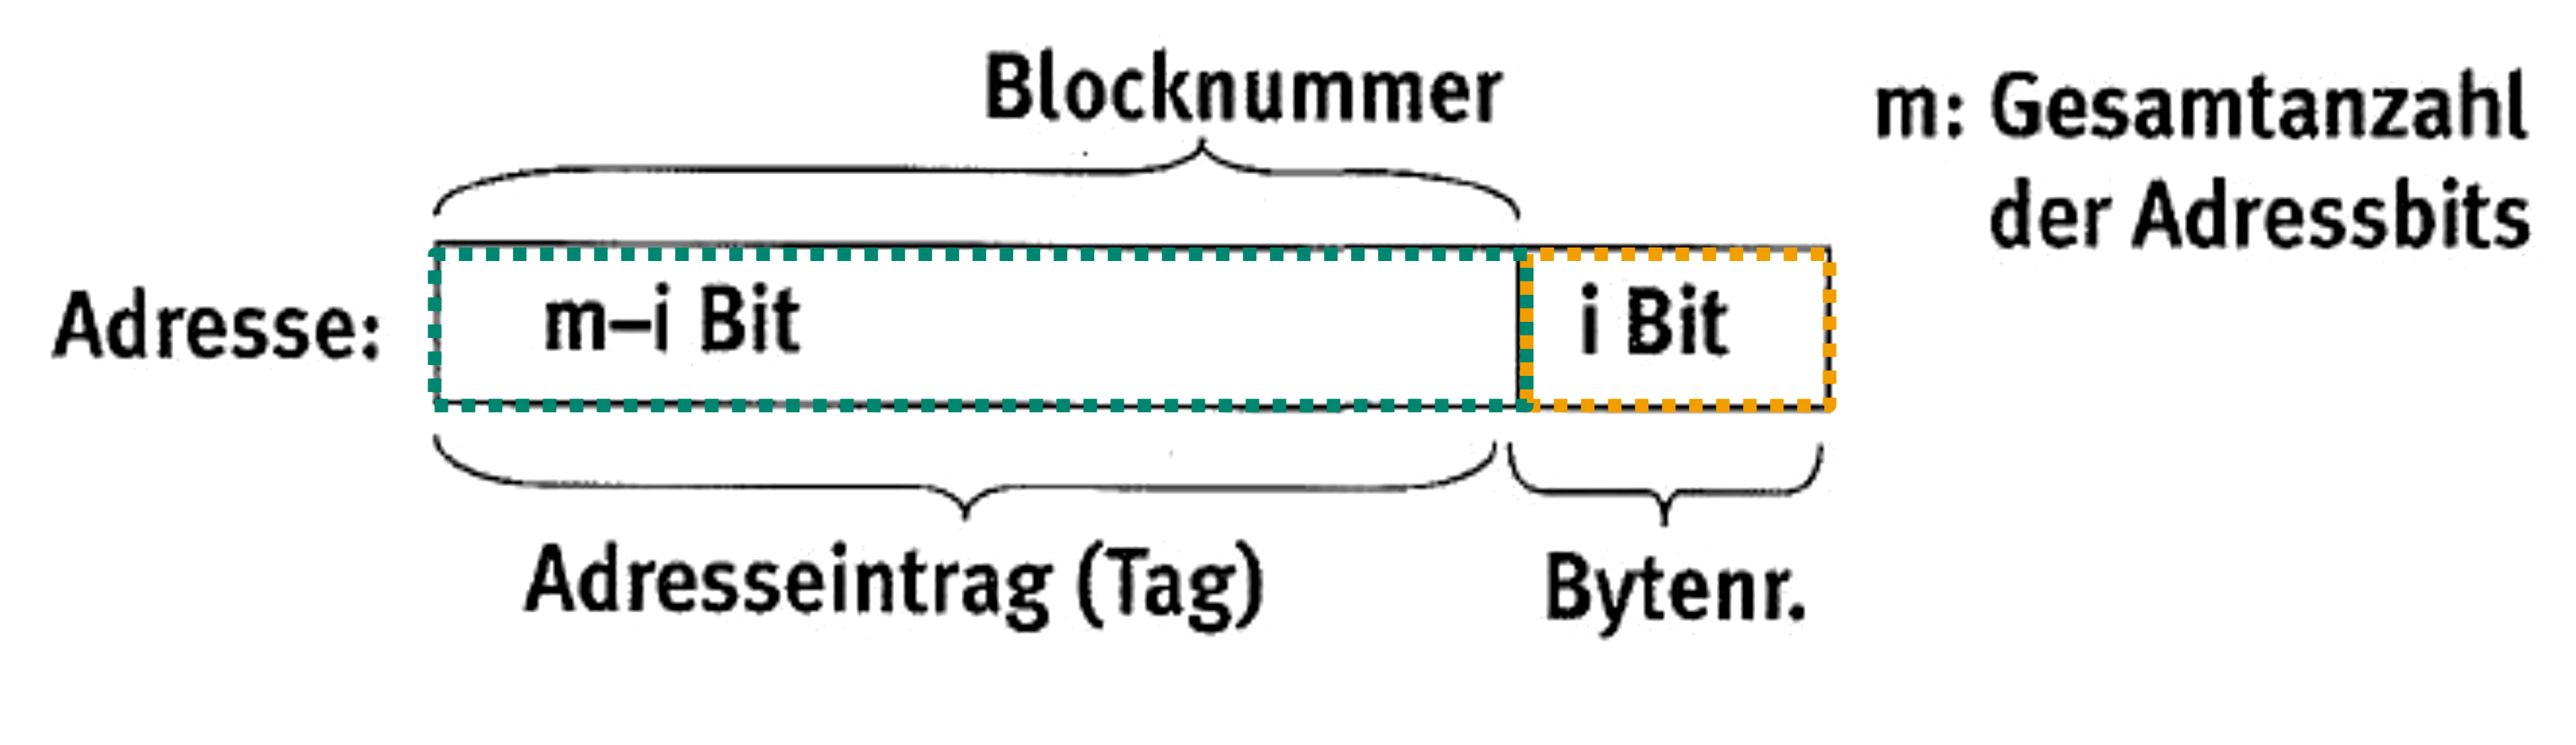
\includegraphics[width=.8\linewidth]{cache_vollassoziativ.png}
\end{center}

\subsubsection{Einweg-assoziativ}

Auch \textit{Direct-Mapped Cache} gennant. Eindeutige Abbildung zwischen den Blocknummern und den Cache-Zeilennummern.
Nur noch ein Adressvergleich nötig. Ungünstige Folge von Speicherzugriffen kann ein sehr häufiges Nachladen ergeben.

Übung: Tags in gleicher Zeile jeweils Überschreiben.

Cache Grösse: \formula{$2^{k+i}$}
Anzahl Zeilen: \formula{$2^k$}
Zeilen-Grösse: \formula{$2^i$}

\begin{center}
    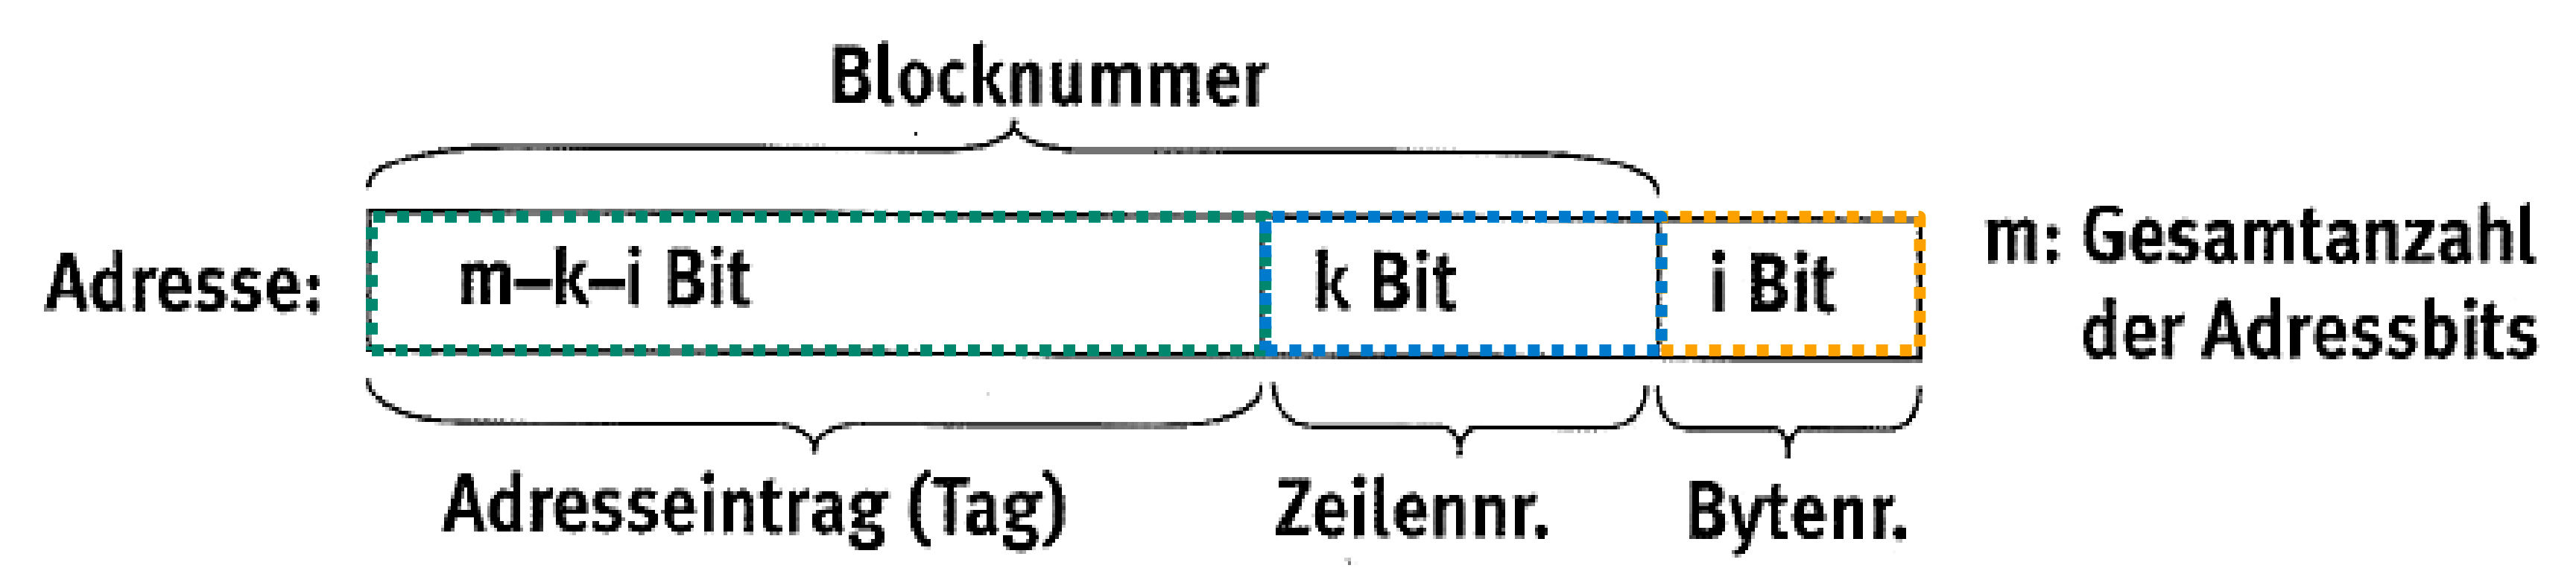
\includegraphics[width=.8\linewidth]{cache_einwegassoziativ.png}
\end{center}

\subsubsection{N-weg assoziativ}

Pro Zeilennummer stehen mehrere Cache-Zeilen zur Auswahl. Jede Cache-Zeile wird n-mal dupliziert.
Es sind insgesamt n Adressvergleiche nötig.

Übung: Wenn Zeile bereits mit anderem Tag belegt, in nächsten Block (n-Way) schreiben.

Cache Grösse: \formula{$n \cdot 2^{k+i}$}
Anzahl Zeilen: \formula{$2^k$}\\
$n$ Blöcke à Zeilen-Grösse: \formula{$2^i$}

\subsection{Ersetzungsstrategien}

\begin{itemize}
    \itemsep-.5em 
    \item LRU (Least Recently Used)
    \item Random Strategie
    \item FIFO (First In First Out)
    \item LFU (Least Frequently Used)
    \item Pseudo-LRU (Siehe Bild)
\end{itemize}

\begin{center}
    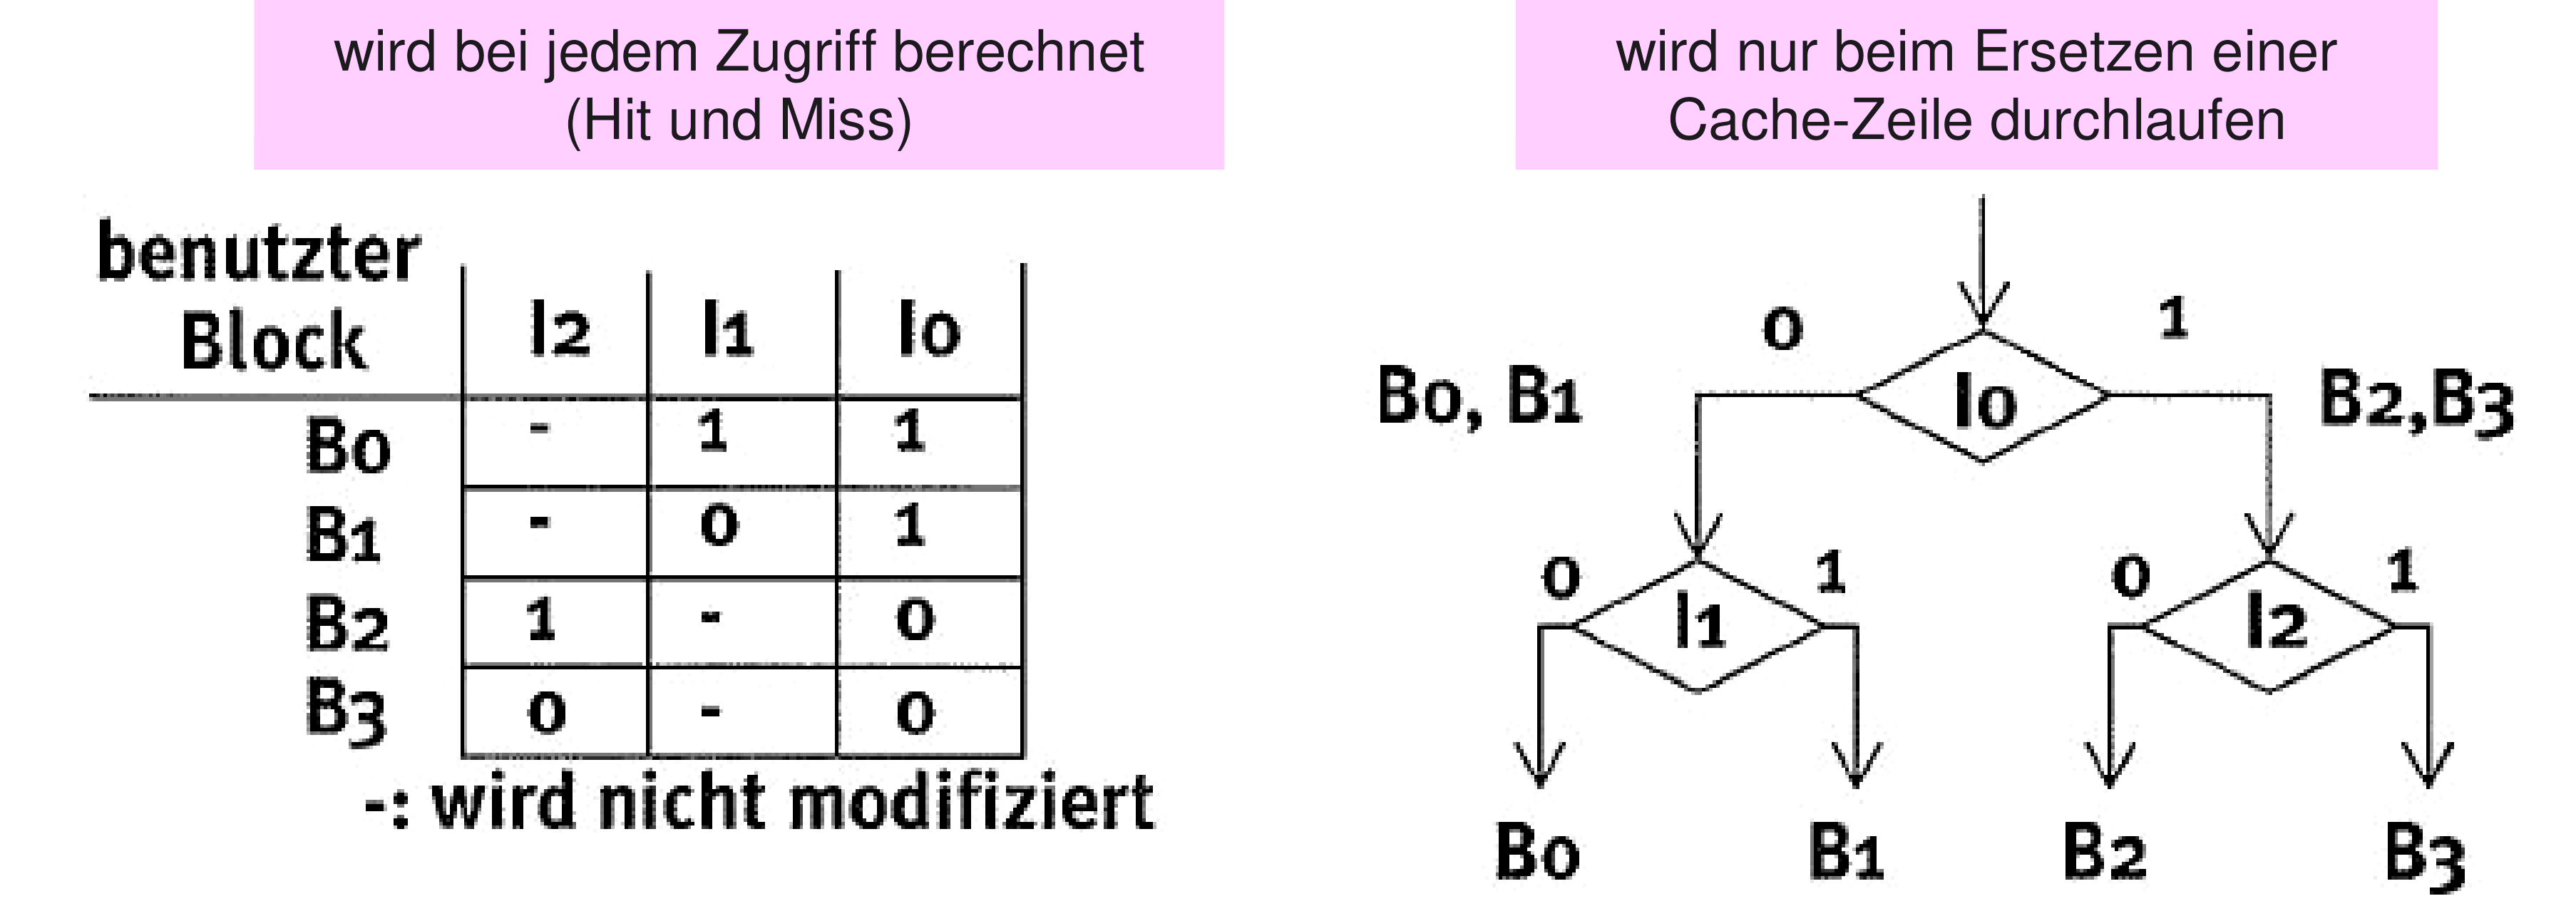
\includegraphics[width=\linewidth]{PLRUexample.png}
\end{center}

\subsection{Schreiben}

\begin{center}
    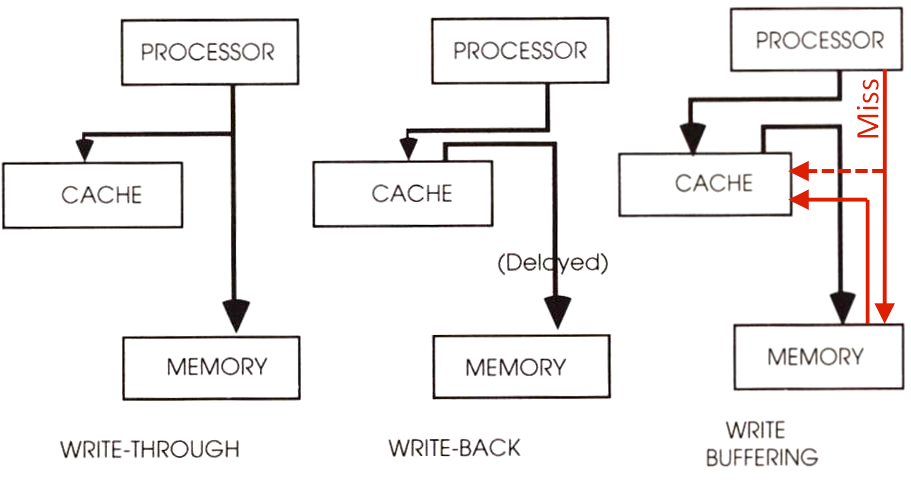
\includegraphics[width=\linewidth]{Cache_Schreiben.png}
\end{center}

\subsubsection{Write Through (Store Through)}

Bei jedem Schreibzyklus werden die Daten in den Hauptspeicher zurückgeschrieben.

\subsubsection{Write Back (Copyback, Store In)}

Bei einem Write-Hit wird nur der Cache-Inhalt neu geschrieben.
Zurückschreiben aller geänderten Cache-Zeilen in den Hauptspeicher wird
durch eine Maschineninstruktion oder Hardware-Signal veranlasst bzw. beim Ersetzen der jeweiligen Cache-Zeile.

\subsubsection{Write Allocate}

Möglichkeiten bei Write-Miss:
\begin{itemize}
    \itemsep-.5em 
    \item No-Write Allocate: Write-Miss verändert Cache nicht; stattdessen direktes Schreiben in Hauptspeicher
    \item Write Allocate: Nachladen der Cache-Zeile (= Read-Miss); danach Verfahren wie bei Write-Hit
\end{itemize}

Typische Kombinationen:
\begin{itemize}
    \itemsep-.5em 
    \item Write Back Cache mit Write Allocate
    \item Write Through Cache mit No-Write Allocate
\end{itemize}

\subsection{Performance}

\formula{$\mathit{Memory\, stall\, cycles} = \mathit{Number\, of\, misses} \cdot \mathit{Miss\, penalty}$}
\formula{$= \mathit{IC} \cdot \dfrac{\mathit{Misses}}{Instructions} \cdot \mathit{Miss\, penalty} $}
\formula{$= \mathit{IC} \cdot \dfrac{\mathit{Memory\, accesses}}{Instructions} \cdot \mathit{Miss\, rate} \cdot \mathit{Miss\, penalty} $}

\formula{$T_{eff} = T_{Hit} + r_{Miss} \cdot A_{Miss}$}

\unitText{$T_{eff}$}{Durchschnittliche Zugriffszeit}{s, Clocks}\\
\unitText{$T_{Hit}$}{Cache zugriffszeit}{s, Clocks}\\
\unitText{$r_{Miss}$}{Miss-Rate im Cache}{\%}\\
\unitText{$A_{Miss}$}{Zusätzlicher Zeitaufwand bei Nichttreffer}{s, Clocks}

\subsection{Cache-Kohärenz}

Das Problem der Cache-Kohärenz kann auf verschiedene Arten gelöst werden:

\begin{itemize}
    \itemsep-.5em 
    \item Gemeinsame Daten werden nicht über den Cache geführt.
    \item Alle Caches arbeiten nach der Write Through-Strategie.
    \item Für alle Cache-Strategien ist die Anwendung eines Kohärenzprotokolls möglich.
\end{itemize}

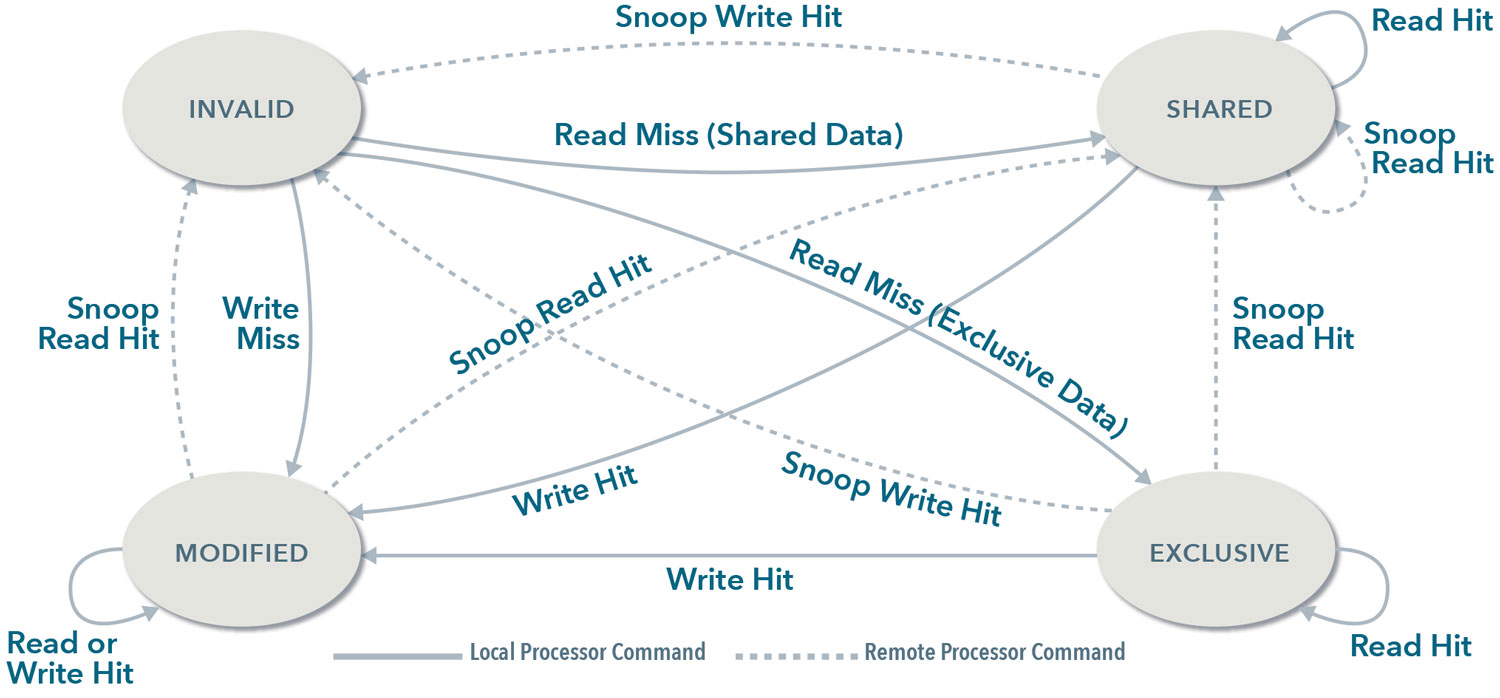
\includegraphics[width=\linewidth]{MESI_Kohaerenz_Protokoll.jpg}


\subsection{Cache-Friendly Code}

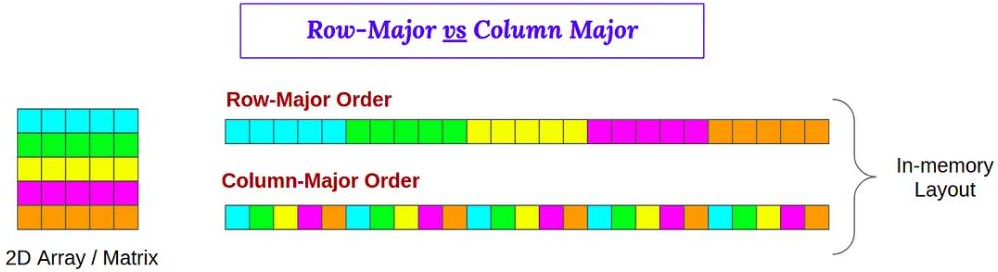
\includegraphics[width=\linewidth]{cache_friendly_code_2.png}
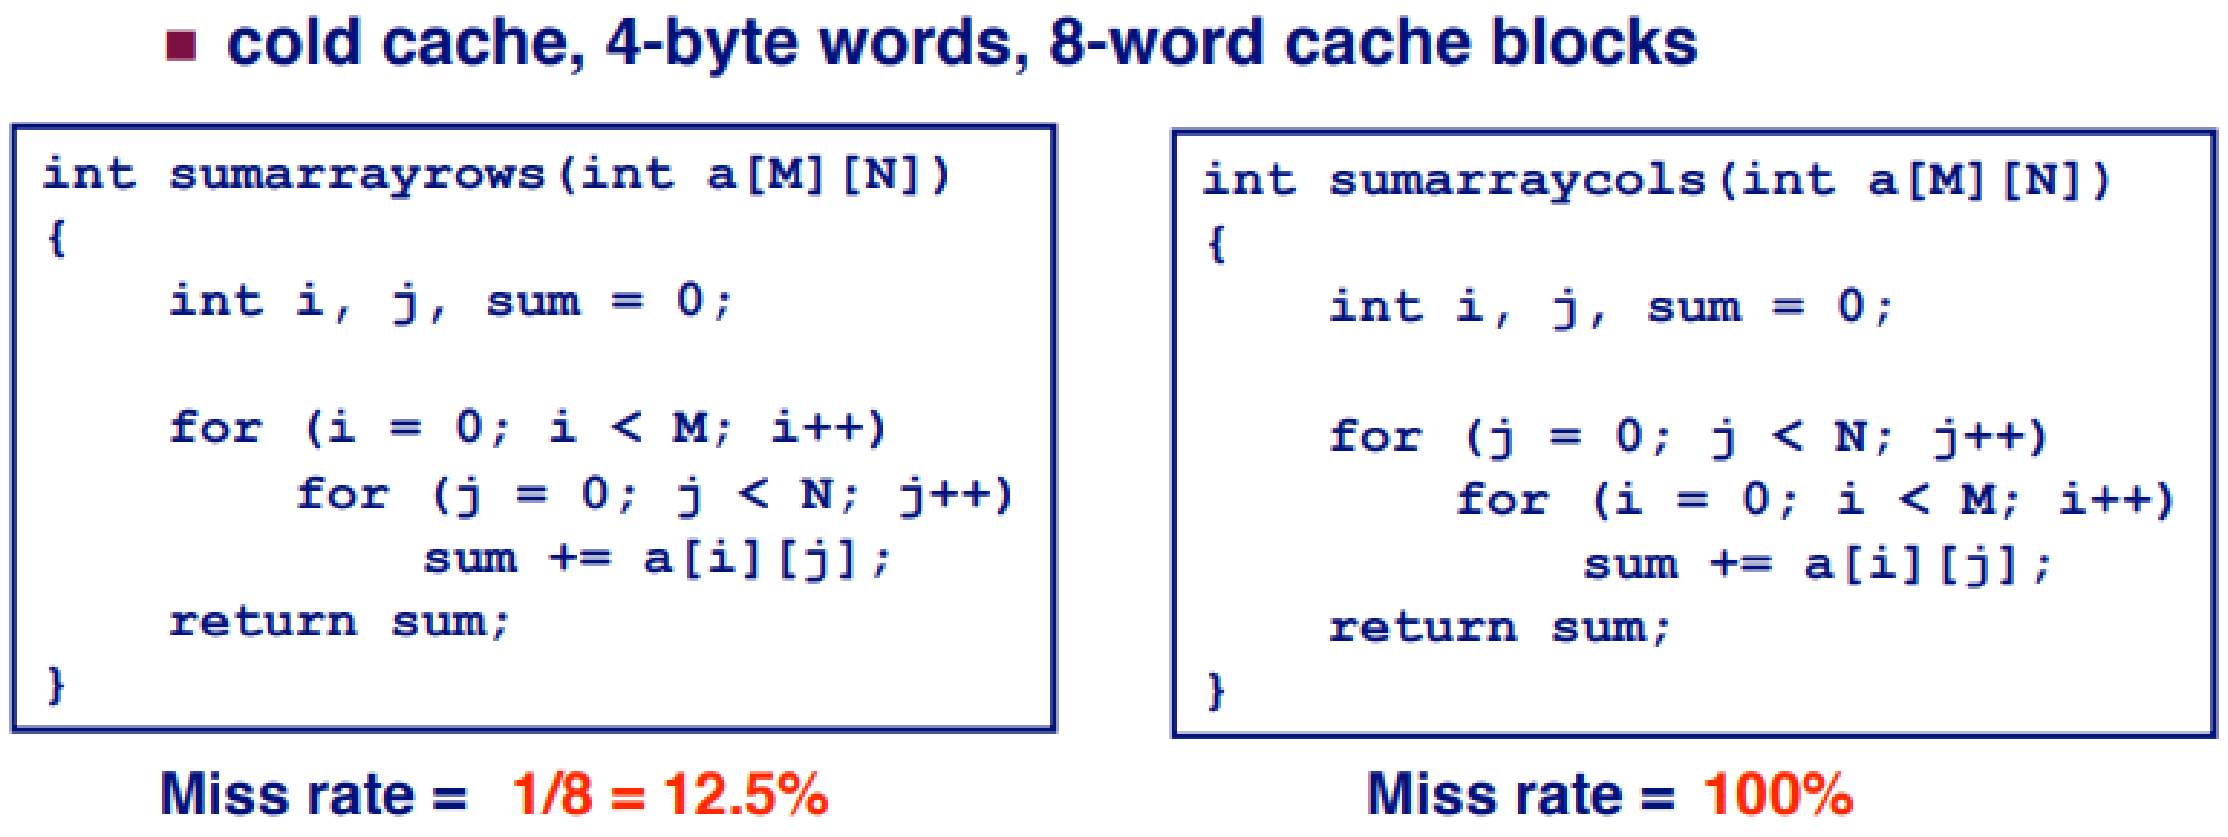
\includegraphics[width=\linewidth]{cache_friendly_code_1.png}
	\section{Adresstransformation}

\textbf{Logischer Cache}: Cache über logische Adressen ansprechen. Adresstransformation erfolgt nach dem Cache.

\textbf{Physischer Cache}: Cache über physische Adressen ansprechen. Adresstransformation erfolgt vor dem Cache.


Zwei Ansätze:

\textbf{Page-Transformation}: Aufteilen des physischen Speichers in Seiten (Pages) einheitlicher Grösse.

\textbf{Segment-Transformation} (Segmentierung): Aufteilen des physischen Speichers in Bereiche (Segments) flexibler Grösse (Grösse von OS bestimmt).

\subsection{Einstufige Page-Transformation}

Pages haben eine feste Länge von $2^k$ Byte.
Die relative Adresse innerhalb einer Page ab Seitenanfang wird \textit{Page-Offset} genannt.
Zuordnung von logischen auf physische Pages erfolgt via \textit{Page-Descriptor-Tables} (Umsetzungstabellen) in der MMU.

{\scriptsize
$n$: Anazahl Bit der physischen Adresse\\
$m$: Anazahl Bit der logischen Adresse\\
$k$: Anazahl Bit des Page-Offsets\\
$x$: LS-Bit der physischen Page-Nummer im Page-Desktiptor\\
$A_p$: Physische Adresse (Speicheradresse)\\
$A_L$: Logische Adresse (Programmadresse, effektive Adresse)\\
$PD$: Umsetztabelle (Einträge sind die Page-Deskrptoren)\\
$PD[i]$: Page Desktiptoren-Nummer $i$ (Eintrag im Index $i$ aus $PD$)\\
|: Aneinanderfügen von Bitmuster (Concatenation)\\
<$i$..$j$>: Bit-Positionen aus einem Bitmuster\\
$+$: Addition von Bitmuster
}

\formula{$A_p$<$n$-1..0> = $PD$[$A_L$ <$m$-1..$k$>]<$x$+($n$-1-$k$)..$x$>|$A_L$<$k$-1..0>}

\begin{center}
    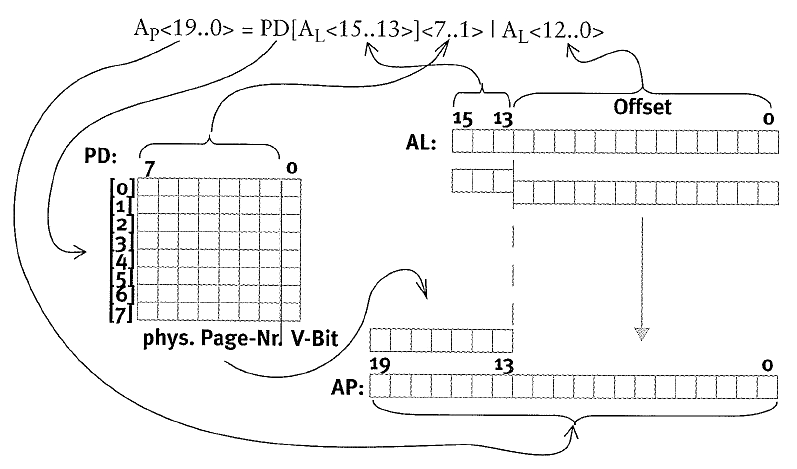
\includegraphics[width=\linewidth]{PageTransformationsformel.png}
    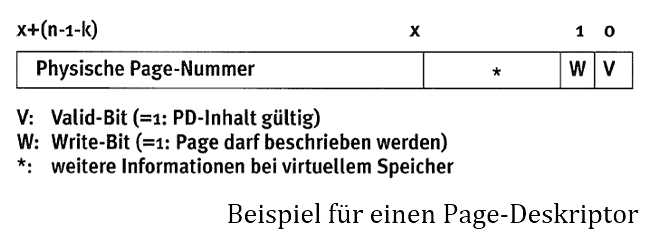
\includegraphics[width=\linewidth]{PageDeskriptor.png}
\end{center}


\subsection{Mehrstufige Page-Transformation}

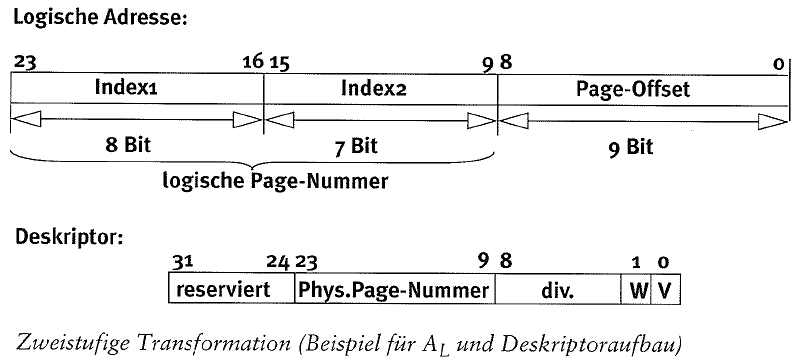
\includegraphics[width=\linewidth]{MehrstufigePagetransformation.png}
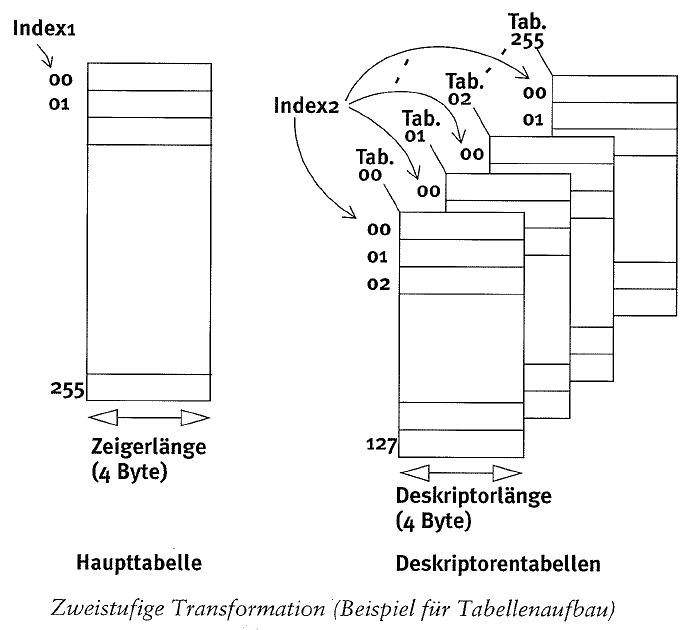
\includegraphics[width=\linewidth]{MehrstufigeTransformation.png}


\section{Virtueller Speicher}

Virtualisierun gerlaubt Ausführung von Programmen, die nicht vollständig in Hauptspeicher geladen sind. Basierend auf Paging.

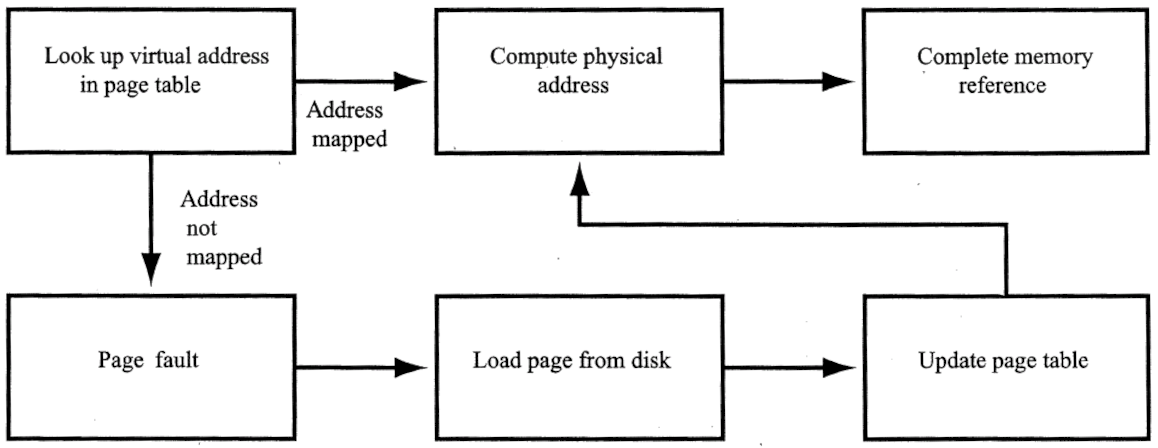
\includegraphics[width=\linewidth]{MMU.png}


\section{Prozessorleistung}

\subsection{Rechenleistung}

\formula{$\mathit{Time} = \dfrac{\mathit{Seconds}}{\mathit{Program}} = \dfrac{\mathit{Instructions}}{\mathit{Program}} \cdot \dfrac{\mathit{Clock cycles}}{Instruction} \cdot \dfrac{\mathit{Seconds}}{\mathit{Clock cycle}}$}

\subsection{Speed-up gemäss Amdahl's Law}

\formula{$T_m = T_s + T_p = \dfrac{s \cdot A}{L_{SISD}} + \dfrac{p \cdot A}{n \cdot L_{SISD}} = \dfrac{A}{L_{SISD}} \cdot (s + \dfrac{p}{n})$}
\formula{$\mathit{Speedup} = \dfrac{L_{MIMD}}{L_{SISD}} = \dfrac{1}{s + \dfrac{1 - s}{n}}$}
	
	\newpage
\onecolumn

\section{Code Beispiele}

\subsection{Software Timer}

\underline{Software Timer API}
\lstinputlisting[firstline=0,lastline=30,style=cppstyle]{./Code/SoftwareTimer_API.c}

\underline{PWM LED}
\lstinputlisting[firstline=0,lastline=30,style=cppstyle]{./Code/SoftwareTimerPWMLED.c}


\subsection{Management von Tasks} \label{sec:task_management}

\underline{Tasks API}
\lstinputlisting[firstline=0,lastline=60,style=cppstyle]{./Code/TaskManagement_API.c}

\underline{Periodic and Aperiodic Tasks Example}
\lstinputlisting[firstline=0,lastline=60,style=cppstyle]{./Code/ManagementTasks.c}

\subsection{Semaphore} \label{sec:semaphore_api}

\underline{Semaphore API}
\lstinputlisting[firstline=0,lastline=30,style=cppstyle]{./Code/Semaphore_API.c}

\end{document}


